\documentclass[compress]{beamer}
\usepackage{ifthen,verbatim}

\title{Effect of muon alignment on TeV tracks}
\author{Jim Pivarski, Alexei Safonov}
\institute{Texas A\&M University}
\date{ 4 October, 2007}

\newcommand{\isnote}{}
\xdefinecolor{lightyellow}{rgb}{1.,1.,0.25}
\xdefinecolor{darkblue}{rgb}{0.1,0.1,0.7}

%% Uncomment this to get annotations
%% \def\notes{\addtocounter{page}{-1}
%%            \renewcommand{\isnote}{*}
%% 	   \beamertemplateshadingbackground{lightyellow}{white}
%%            \begin{frame}
%%            \frametitle{Notes for the previous page (page \insertpagenumber)}
%%            \itemize}
%% \def\endnotes{\enditemize
%% 	      \end{frame}
%%               \beamertemplateshadingbackground{white}{white}
%%               \renewcommand{\isnote}{}}

%% Uncomment this to not get annotations
\def\notes{\comment}
\def\endnotes{\endcomment}

\setbeamertemplate{navigation symbols}{}
\setbeamertemplate{headline}{\includegraphics[height=1 cm]{../cmslogo} \hspace{0.1 cm} \includegraphics[height=1 cm]{../tamulogo} \hfill
\begin{minipage}{5.5 cm}
\vspace{-0.75 cm} \small
\begin{center}
\ifthenelse{\equal{\insertpagenumber}{1}}{}{\textcolor{blue}{\insertsection}}
\end{center}
\end{minipage} \hfill
\begin{minipage}{4.5 cm}
\vspace{-0.75 cm} \small
\begin{flushright}
\ifthenelse{\equal{\insertpagenumber}{1}}{}{Jim Pivarski \hspace{0.5 cm} \insertpagenumber\isnote/\pageref{numpages}}
\end{flushright}
\end{minipage}\mbox{\hspace{0.2 cm}}}

\begin{document}
\frame{\titlepage}

%% \begin{frame}

%% what we're doing and overview: need for a bottom line

%% impact of misalignment on track resolution: baselines first, then
%% fractional worsening of resolution from misalignment only

%% muoncompares

%% compares: only ideal, muonscenario, and tracker1: use same colors

%% first thing to notice: misalignment contributes more significantly to
%% resolution of resonances than smearing of background

%% background-smearing depends exponentially on the Gaussian width of
%% tail contributions; how close are we to the tipping point?  Not close
%% at all.  We should see large discrepancies in chamber overlaps before
%% background-smearing becomes significant

%% so let's concentrate on resonance broadening: define bottom line as
%% RMS of event-by-event ratio

%% \end{frame}

\begin{frame}
\frametitle{Need for a bottom line}
\begin{itemize}
\item We have seen that muon alignment needs surprisingly few tracks
for 100~$\mu$m accuracy RMS in $x$, but
\begin{itemize}
\item some degrees of freedom better aligned than others
\item some distributions have tails, especially systematics studies
\end{itemize}
\begin{center}
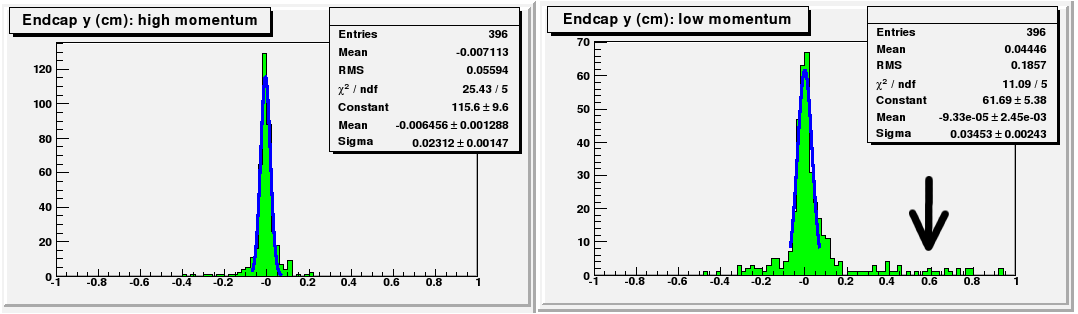
\includegraphics[width=0.9\linewidth]{momentum_accuracy.png}
\end{center}
\item To assess alignment quality, we can look at its effect on TeV-scale tracks
\begin{itemize}
\item effect on momentum resolution for individual tracks
\item broadening of TeV di-muon resonance (RMS misalignment)
\item smearing of Drell-Yan background (higher moments)
\end{itemize}
\end{itemize}
\end{frame}

\section*{Effect on individual tracks}

\begin{frame}
\begin{center}
\Huge \textcolor{blue}{Effect on individual tracks}
\end{center}
\end{frame}

\begin{frame}
\frametitle{Fractional widening of momentum distribution, binned}
\begin{columns}
\column{0.8\linewidth}
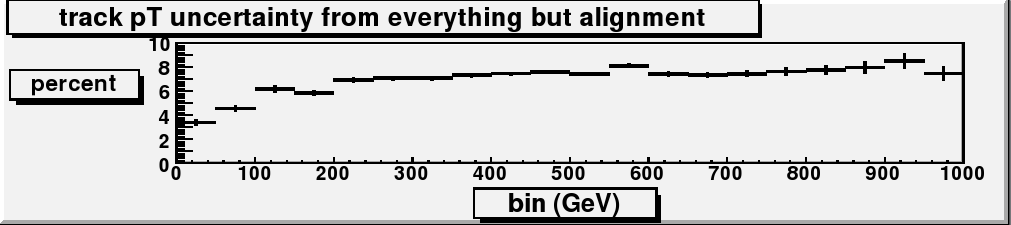
\includegraphics[width=\linewidth]{track_uncertainty_from_all_but_alignment.png}

\only<1>{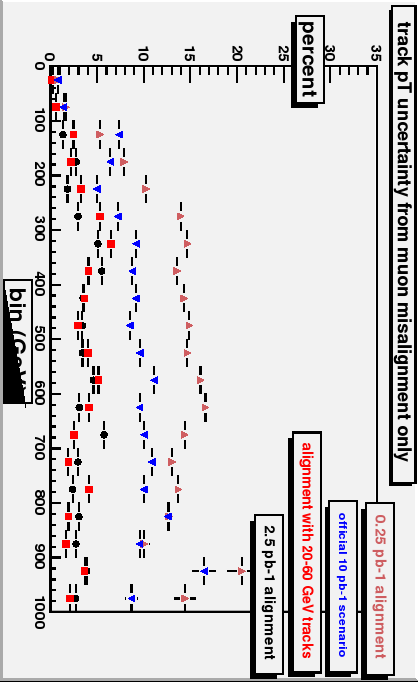
\includegraphics[height=\linewidth, angle=90]{track_uncertainty_from_muon_misalignment.png}}
\only<2>{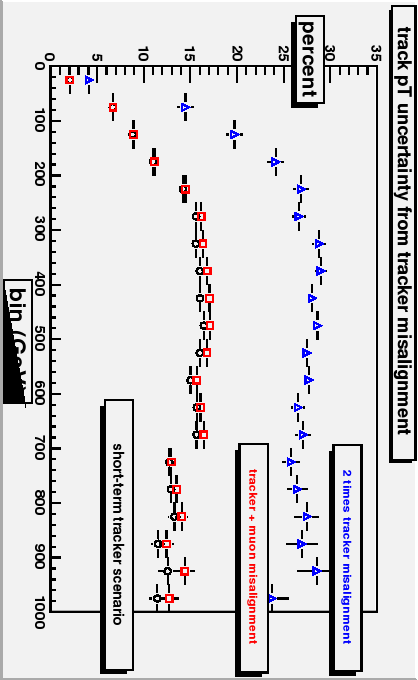
\includegraphics[height=\linewidth, angle=90]{track_uncertainty_from_tracker_misalignment.png}}

\column{0.3\linewidth}
track-by-track RMS

\vspace{0.1 cm}
of $\displaystyle \frac{{p_T}_{\mbox{\scriptsize ideal}}}{{p_T}_{\mbox{\scriptsize generated}}} - 1$

\vspace{0.75 cm}
track-by-track RMS

\vspace{0.1 cm}
of $\displaystyle \frac{{p_T}_{\mbox{\scriptsize misaligned}}}{{p_T}_{\mbox{\scriptsize ideal}}} - 1$

\vspace{1.5 cm}
$\displaystyle \bigg(\frac{\sigma_{p_T}}{p_T}\bigg) = \bigg(\frac{\sigma_\kappa}{\kappa}\bigg)$

\vspace{0.1 cm}
\mbox{$=$ sum in quadrature} \mbox{of both uncertainties}
\end{columns}
\end{frame}

\begin{notes}
\item The plots on the previous two slides require explanation, which
I hope to give verbally when I present this talk (this page is for
archival reference).
\begin{itemize}
\item ${p_T}_{\mbox{\scriptsize generated}}$ is the generator-level $p_T$
\item ${p_T}_{\mbox{\scriptsize ideal}}$ is the reconstructed $p_T$ with perfect alignment
\item ${p_T}_{\mbox{\scriptsize misaligned}}$ is the reconstructed $p_T$ with realistic alignment
\end{itemize}
\item A single reconstructed muon $p_T$ is $\displaystyle \frac{{p_T}_{\mbox{\scriptsize ideal}}}{{p_T}_{\mbox{\scriptsize generated}}} \times \frac{{p_T}_{\mbox{\scriptsize misaligned}}}{{p_T}_{\mbox{\scriptsize ideal}}}$
\item By plotting the RMS of each distribution, I plot
\begin{itemize}
\item the uncertainty in a track $p_T$ due to detector effects other than alignment
\item the uncertainty in a track $p_T$ due to alignment
\end{itemize}
\item Total uncertainty, $\displaystyle \bigg(\frac{\sigma_{p_T}}{p_T}\bigg)\mbox{, which is }\bigg(\frac{\sigma_\kappa}{\kappa}\bigg)$, is the sum in quadrature of the uncertainty of the two factors
\end{notes}

\section*{Effect on di-muon resolution}

\begin{frame}
\begin{center}
\Huge \textcolor{blue}{Effect on di-muon resolution}
\end{center}
\end{frame}

\begin{frame}
\frametitle{Overlay of \only<1>{1}\only<2>{2} TeV Drell-Yan and $Z'$ resonance}
\begin{columns}
\column{0.5\linewidth}
\only<1>{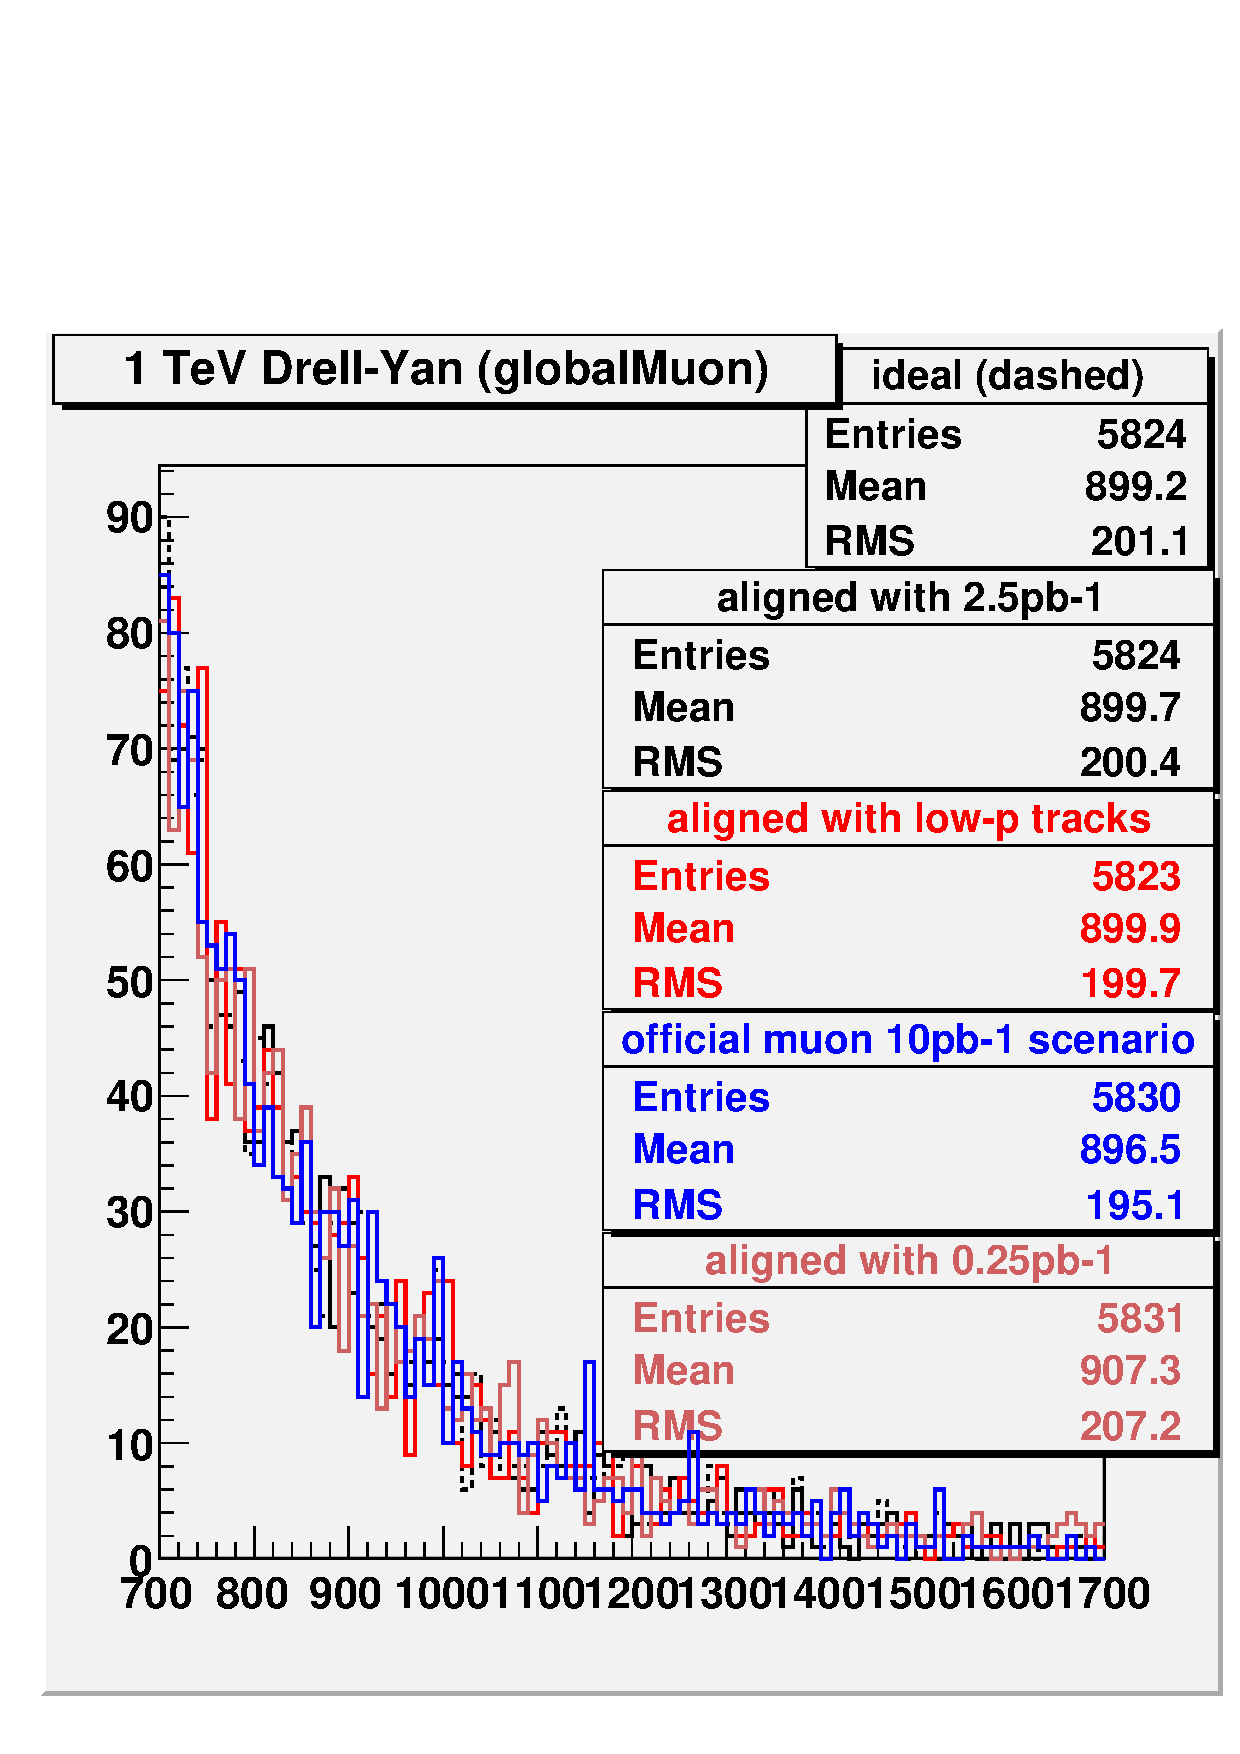
\includegraphics[width=\linewidth]{muoncompare_dy_500.pdf}}
\only<2>{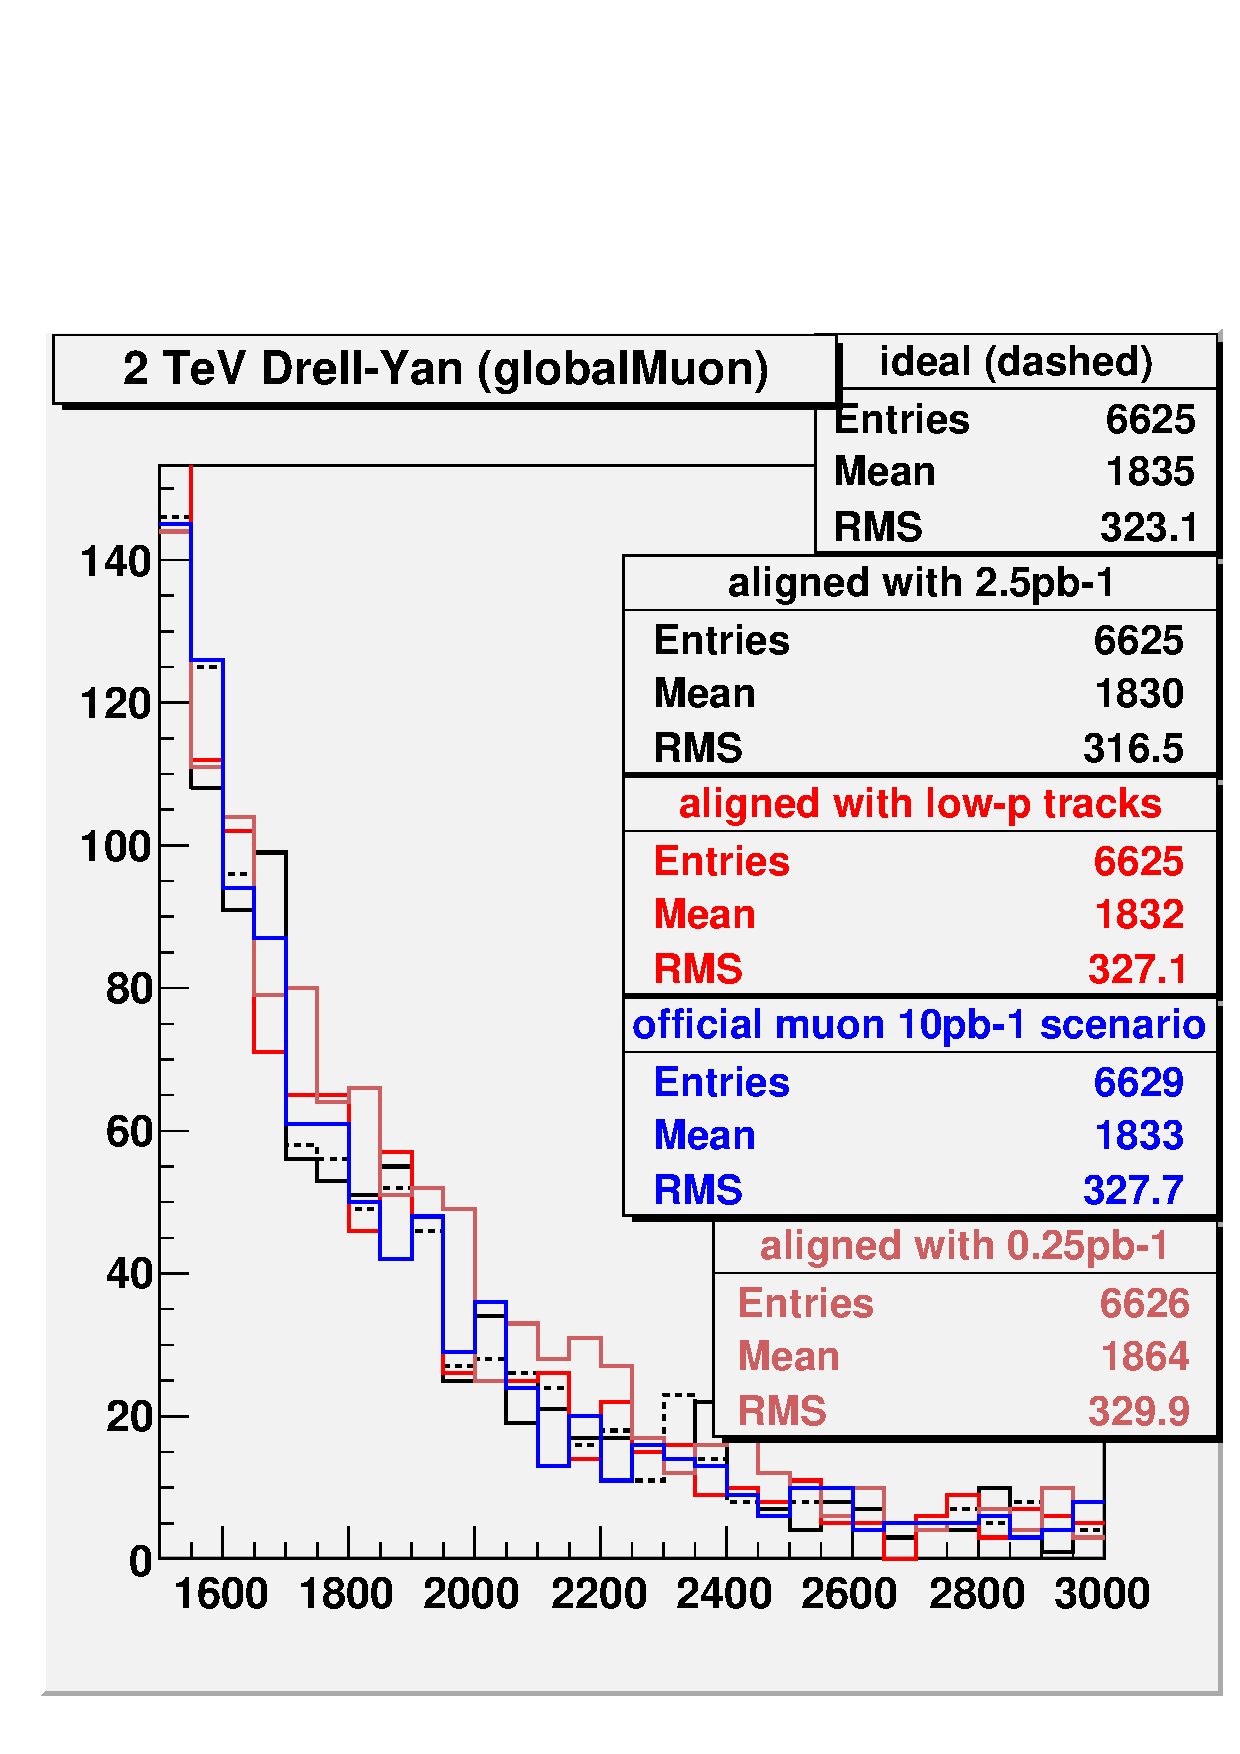
\includegraphics[width=\linewidth]{muoncompare_dy_1000.pdf}}
\column{0.5\linewidth}
\only<1>{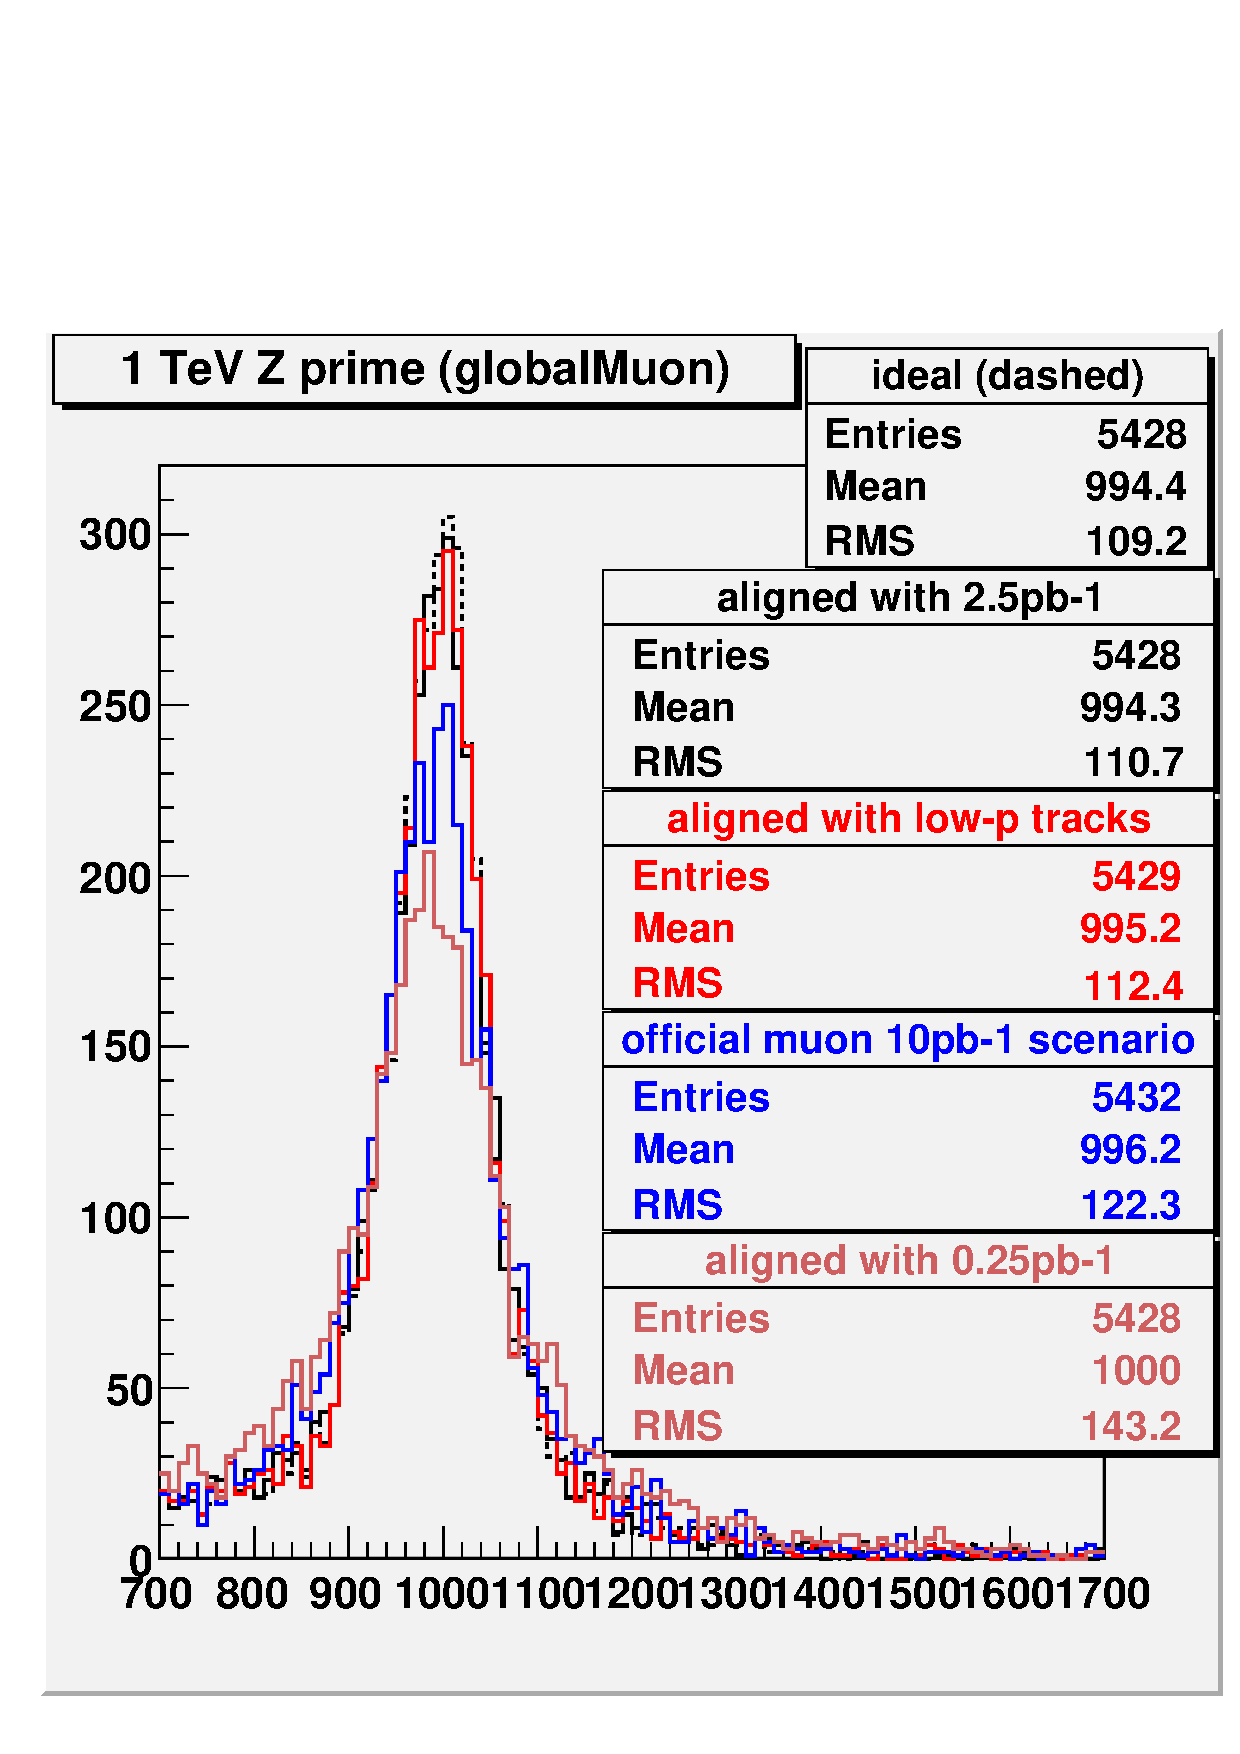
\includegraphics[width=\linewidth]{muoncompare_zprime_1000.pdf}}
\only<2>{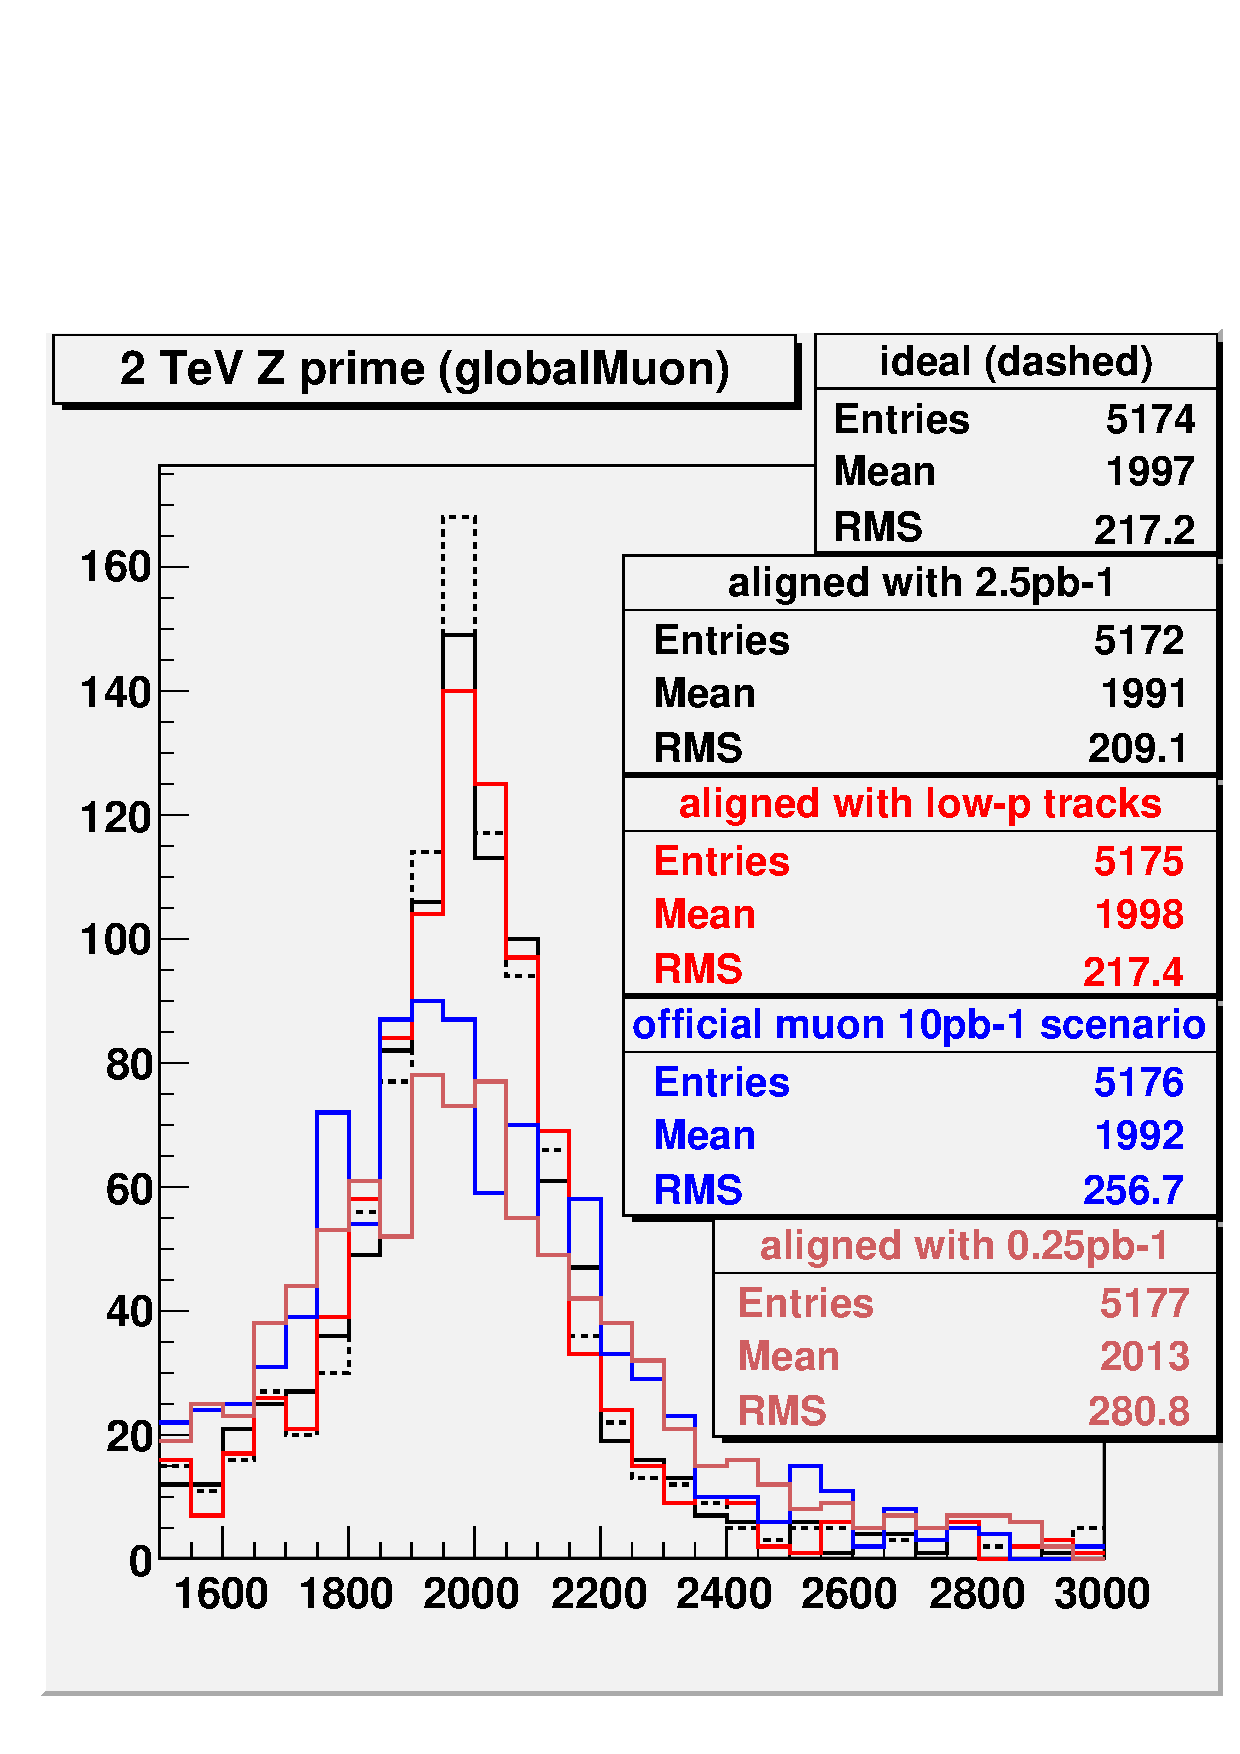
\includegraphics[width=\linewidth]{muoncompare_zprime_2000.pdf}}
\end{columns}

\vspace{0.25 cm}
\textcolor{red}{``low-p'' means 20-60~GeV $Z\to\mu\mu$}

\textcolor{blue}{official 10~pb$^{-1}$ scenario is pessimistic}
\end{frame}

\begin{frame}
\frametitle{Comparison with tracker alignment scenario}
\begin{columns}
\column{0.5\linewidth}
\only<1>{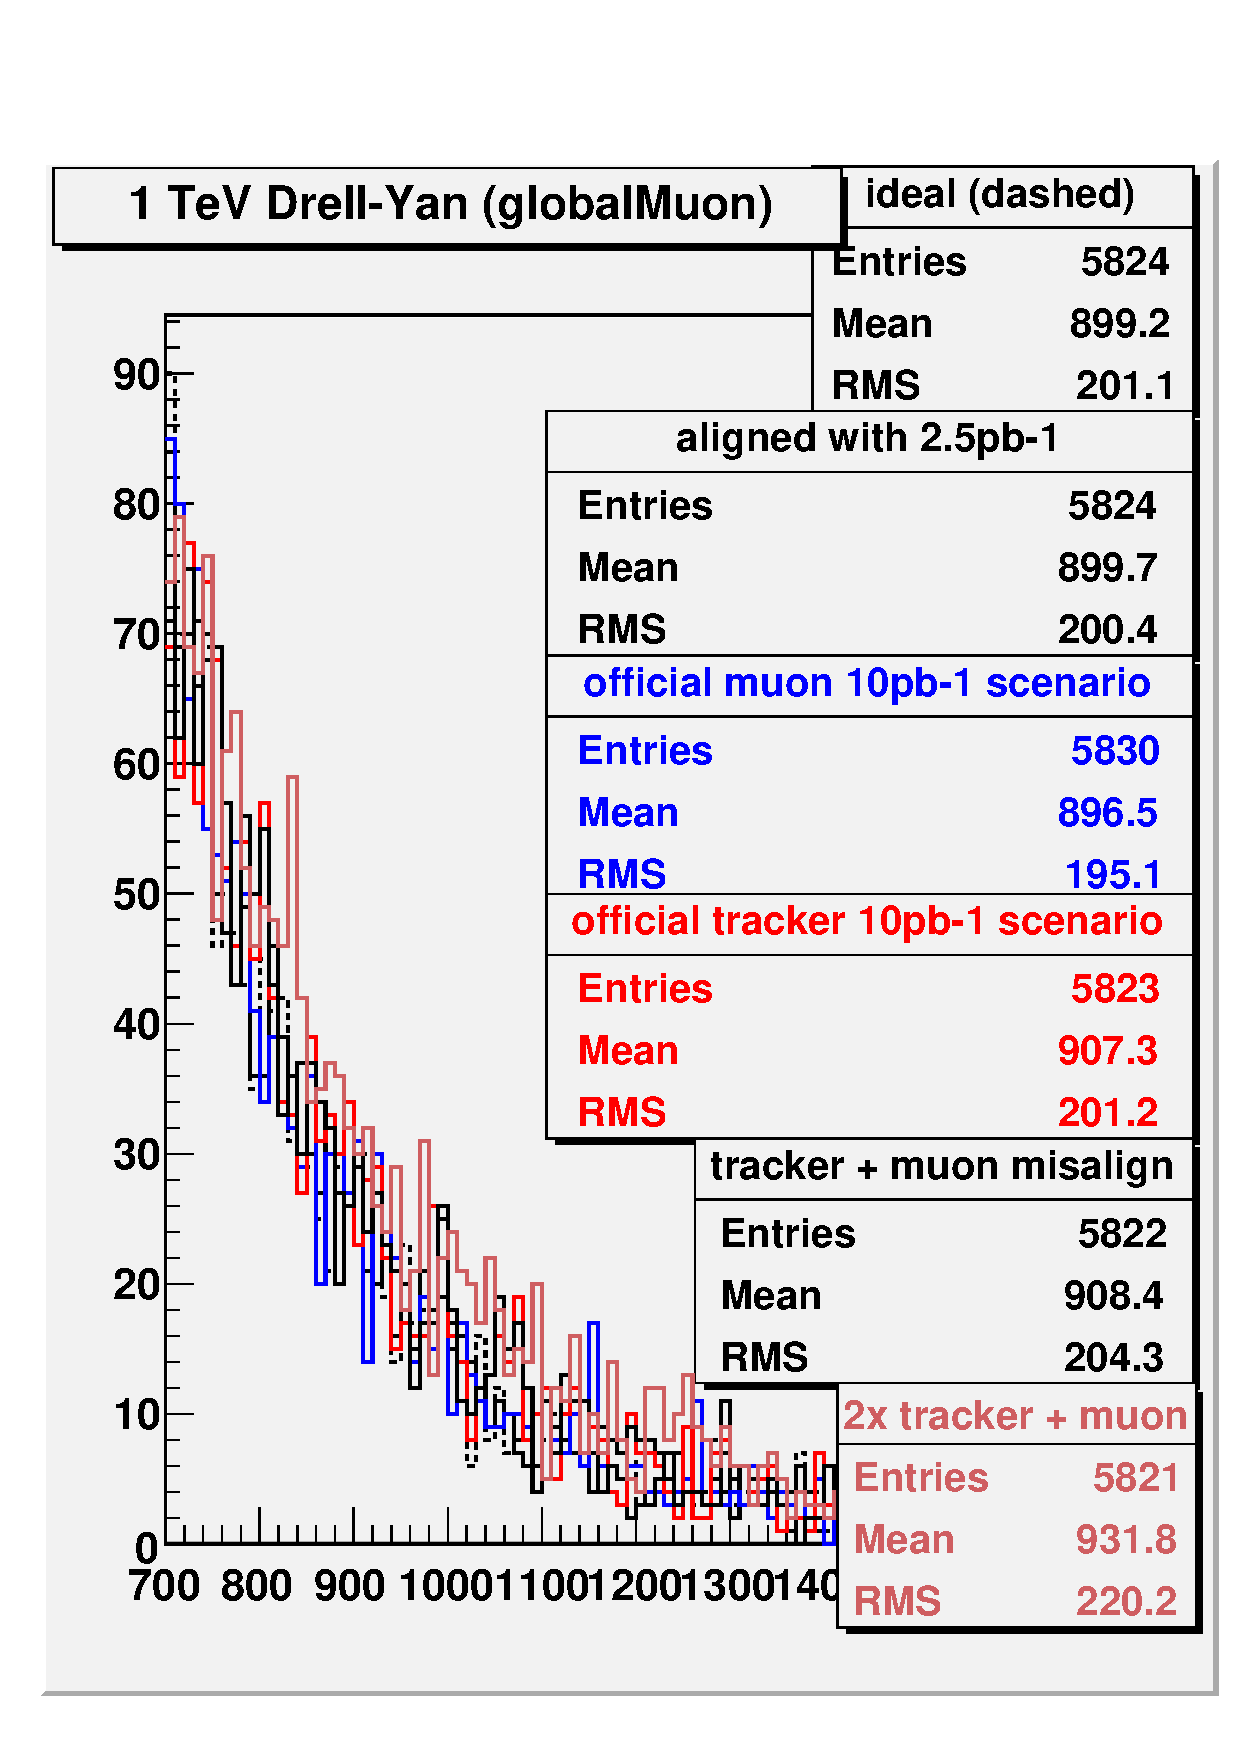
\includegraphics[width=\linewidth]{trackercompare_dy_500.pdf}}
\only<2>{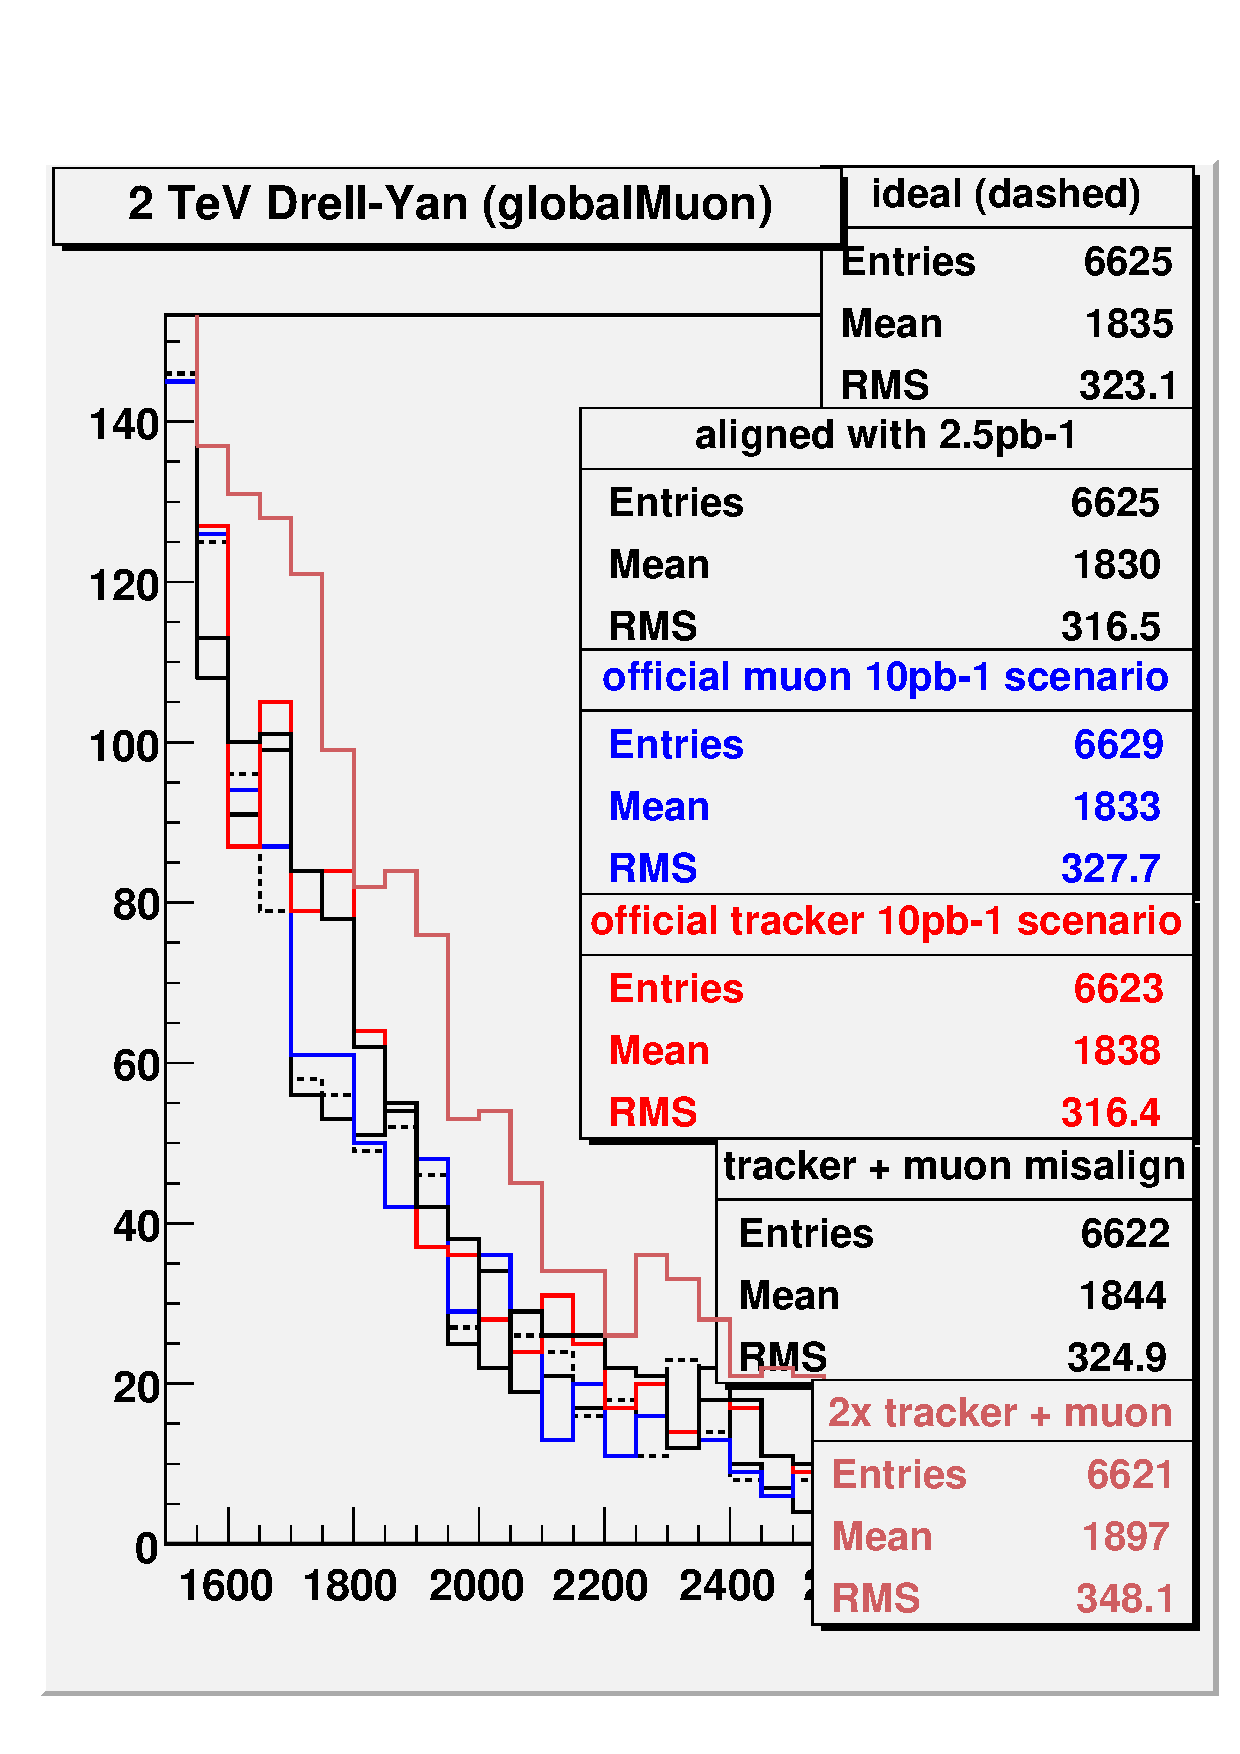
\includegraphics[width=\linewidth]{trackercompare_dy_1000.pdf}}
\column{0.5\linewidth}
\only<1>{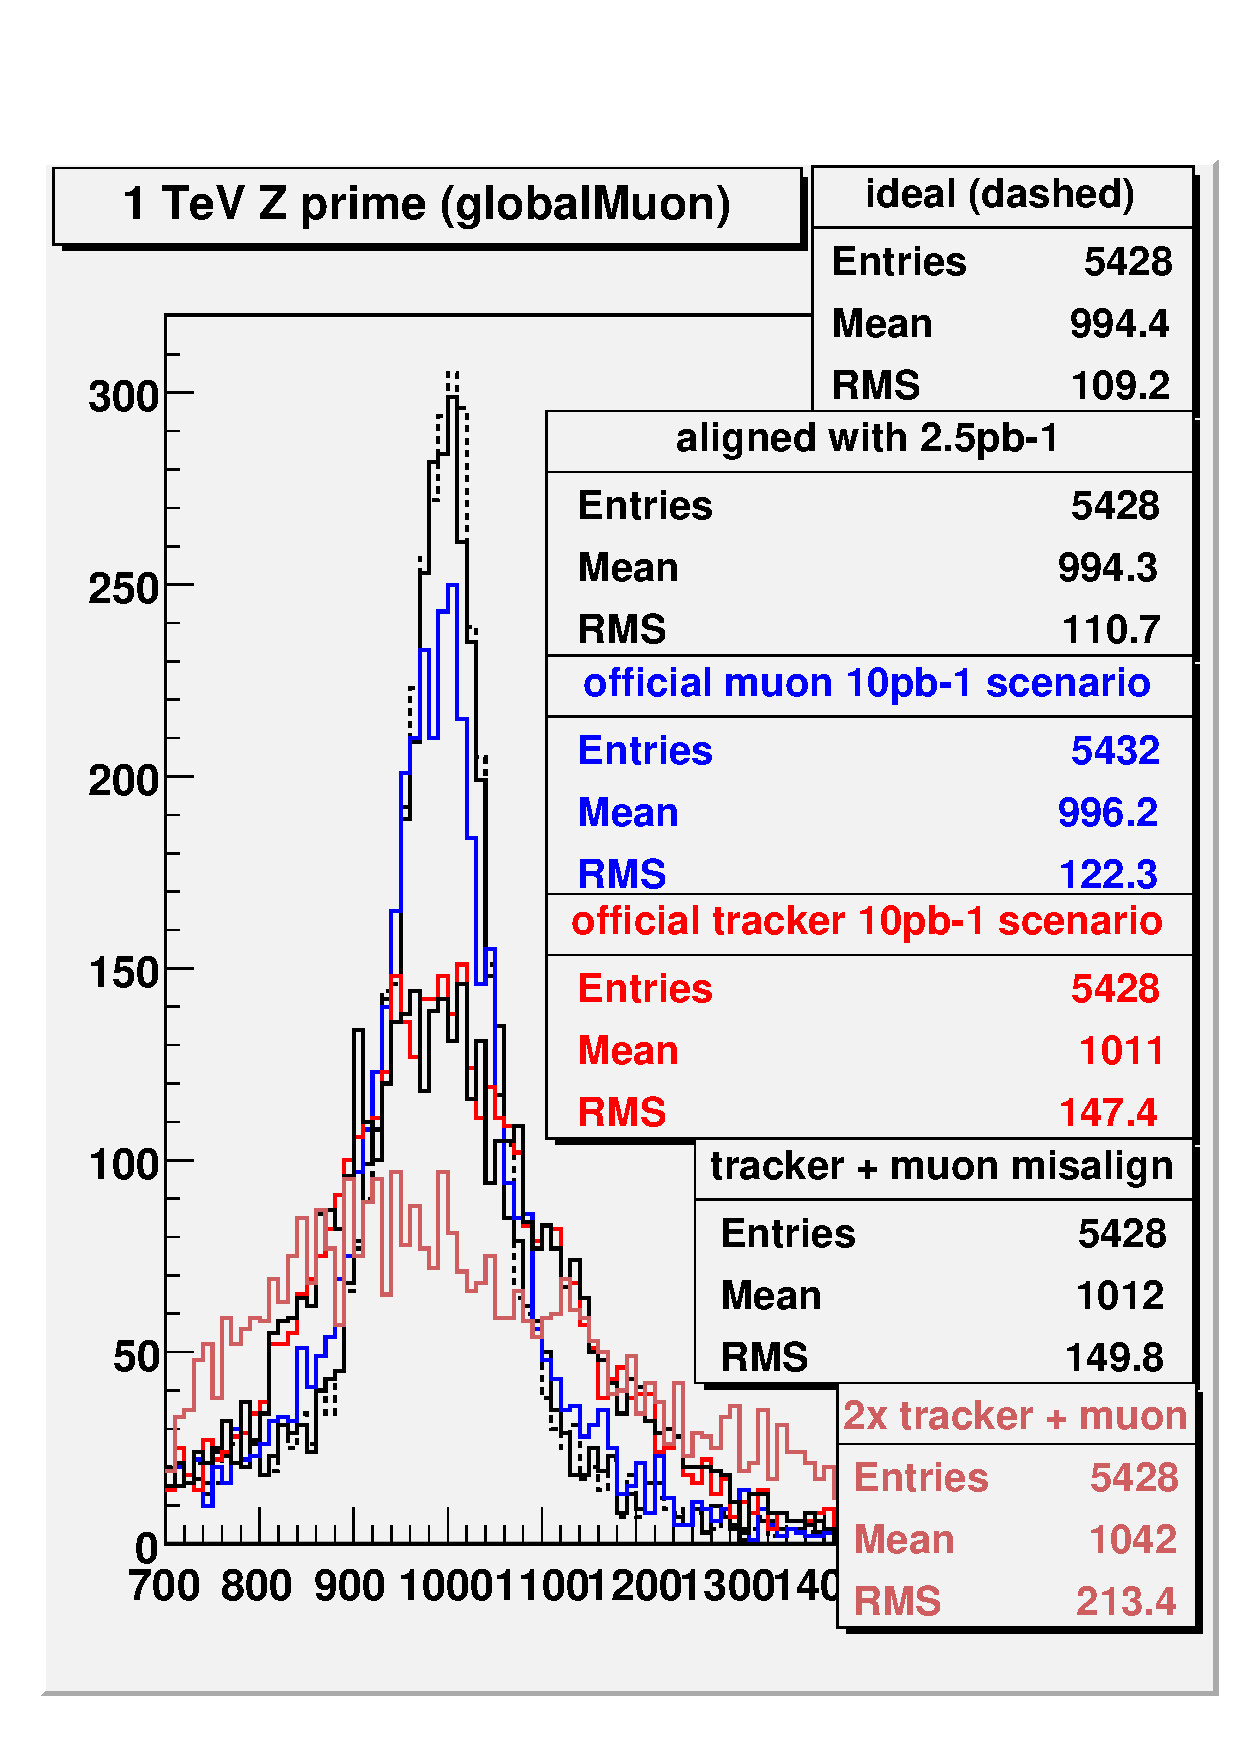
\includegraphics[width=\linewidth]{trackercompare_zprime_1000.pdf}}
\only<2>{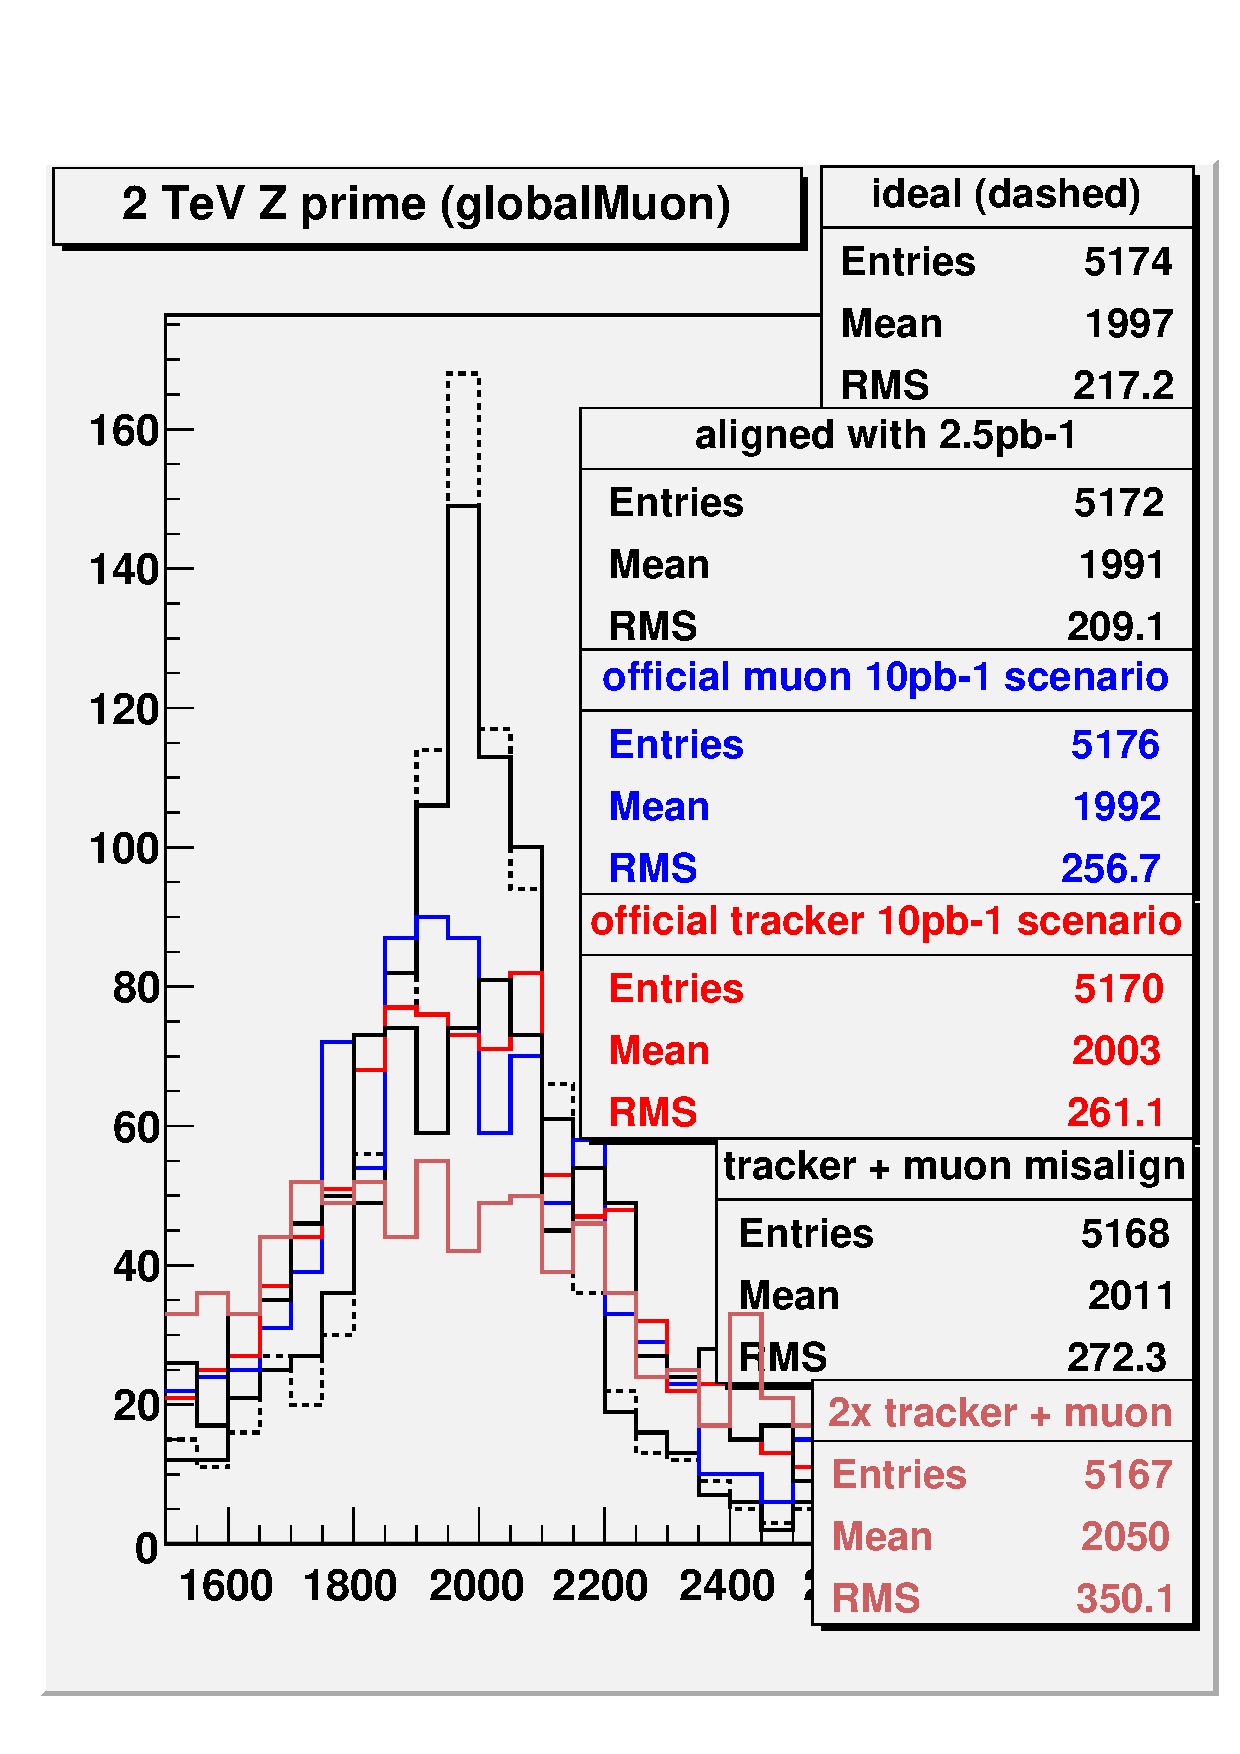
\includegraphics[width=\linewidth]{trackercompare_zprime_2000.pdf}}
\end{columns}

\vspace{0.25 cm}
Careful!  Tracker alignment scenario might be pessimistic, too
\end{frame}

\section*{Drell-Yan (not) smearing}

\begin{frame}
\begin{center}
\Huge \textcolor{blue}{Drell-Yan (not) smearing}
\end{center}
\end{frame}

\begin{frame}
\frametitle{Simple model of Drell-Yan smearing}
\begin{itemize}\setlength{\itemsep}{0.25 cm}
\item<1-> Drell-Yan is exponentially distributed: $f(x) = e^{-kx}$
\item<1-> Convoluted: $\displaystyle f(y) = \int f(x) \, \frac{1}{\sqrt{2\pi}\sigma} \exp\left(\frac{-(x-y)^2}{2\sigma^2}\right) \, dx$
\item<1-> $f(y) = e^{-ky} \, \exp(\sigma^2 k^2 / 2)$
\item<1-> Convolution kernel is a series: $A_1 e^{x^2/2/{\sigma_1}^2} + A_2 e^{x^2/2/{\sigma_2}^2} + \ldots$ (``tails'' are wide Gaussians with small contribution)
\item<1-> $f(y) = e^{-ky} (A_1 \exp({\sigma_1}^2 k^2 / 2) + A_2 \exp({\sigma_2}^2 k^2 / 2) + \ldots)$
\item<1-> Depends linearly on $A_i$ and as $e^{{\sigma_i}^2}$ on width: \fbox{could be big!}
\end{itemize}

\vfill
\begin{itemize}
\item<2->What's $k$ for Drell-Yan? \hfill $k$ = 6$\times$10$^{-3}$/GeV (near 1 TeV) \\ \mbox{ } \hfill and 3.4$\times$10$^{-3}$/GeV (near 2 TeV)
\item<2->What's $\sigma$?
\end{itemize}
\end{frame}

\begin{frame}
\frametitle{Fit Drell-Yan smearing to multi-Gaussian to quantify tail $\sigma$s}
\begin{center}
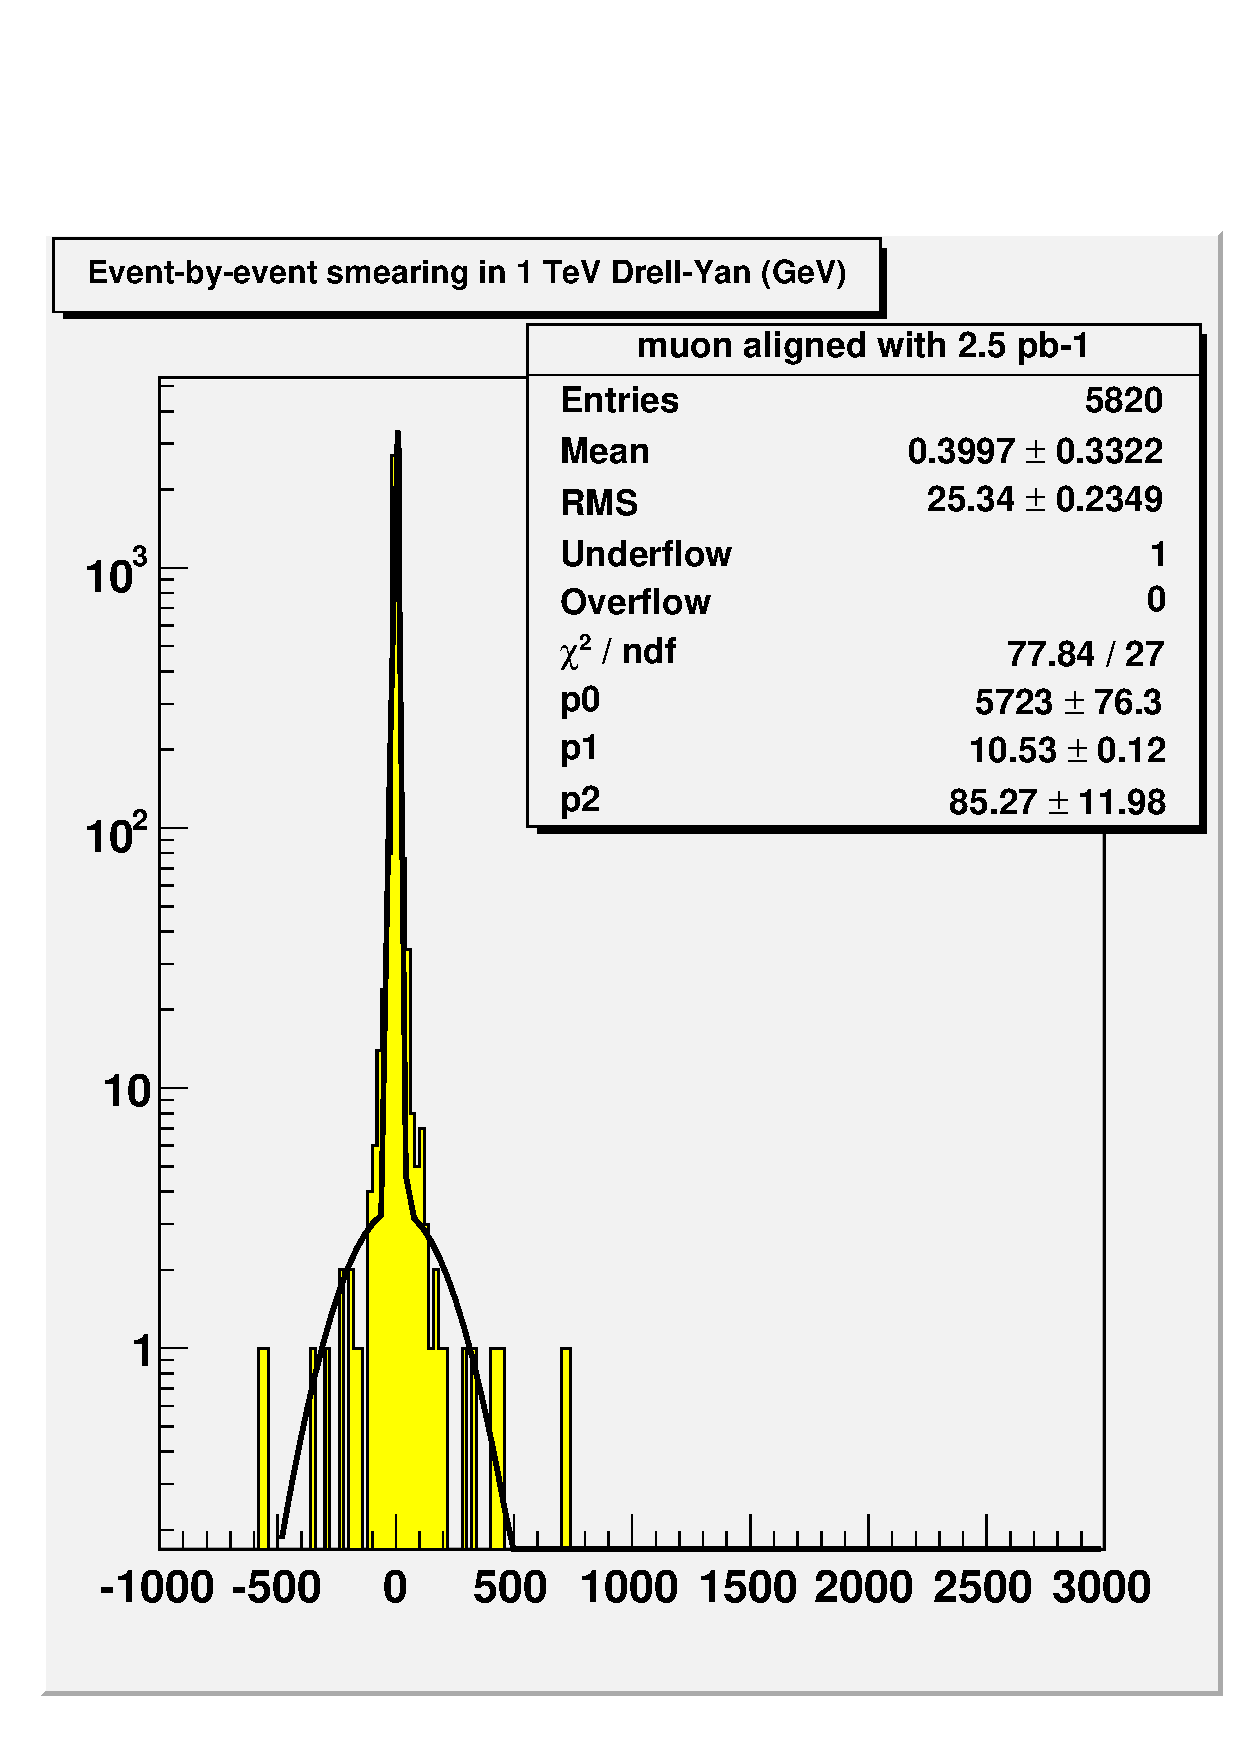
\includegraphics[width=0.33\linewidth]{eventsmear_dy_500_events10k.pdf}
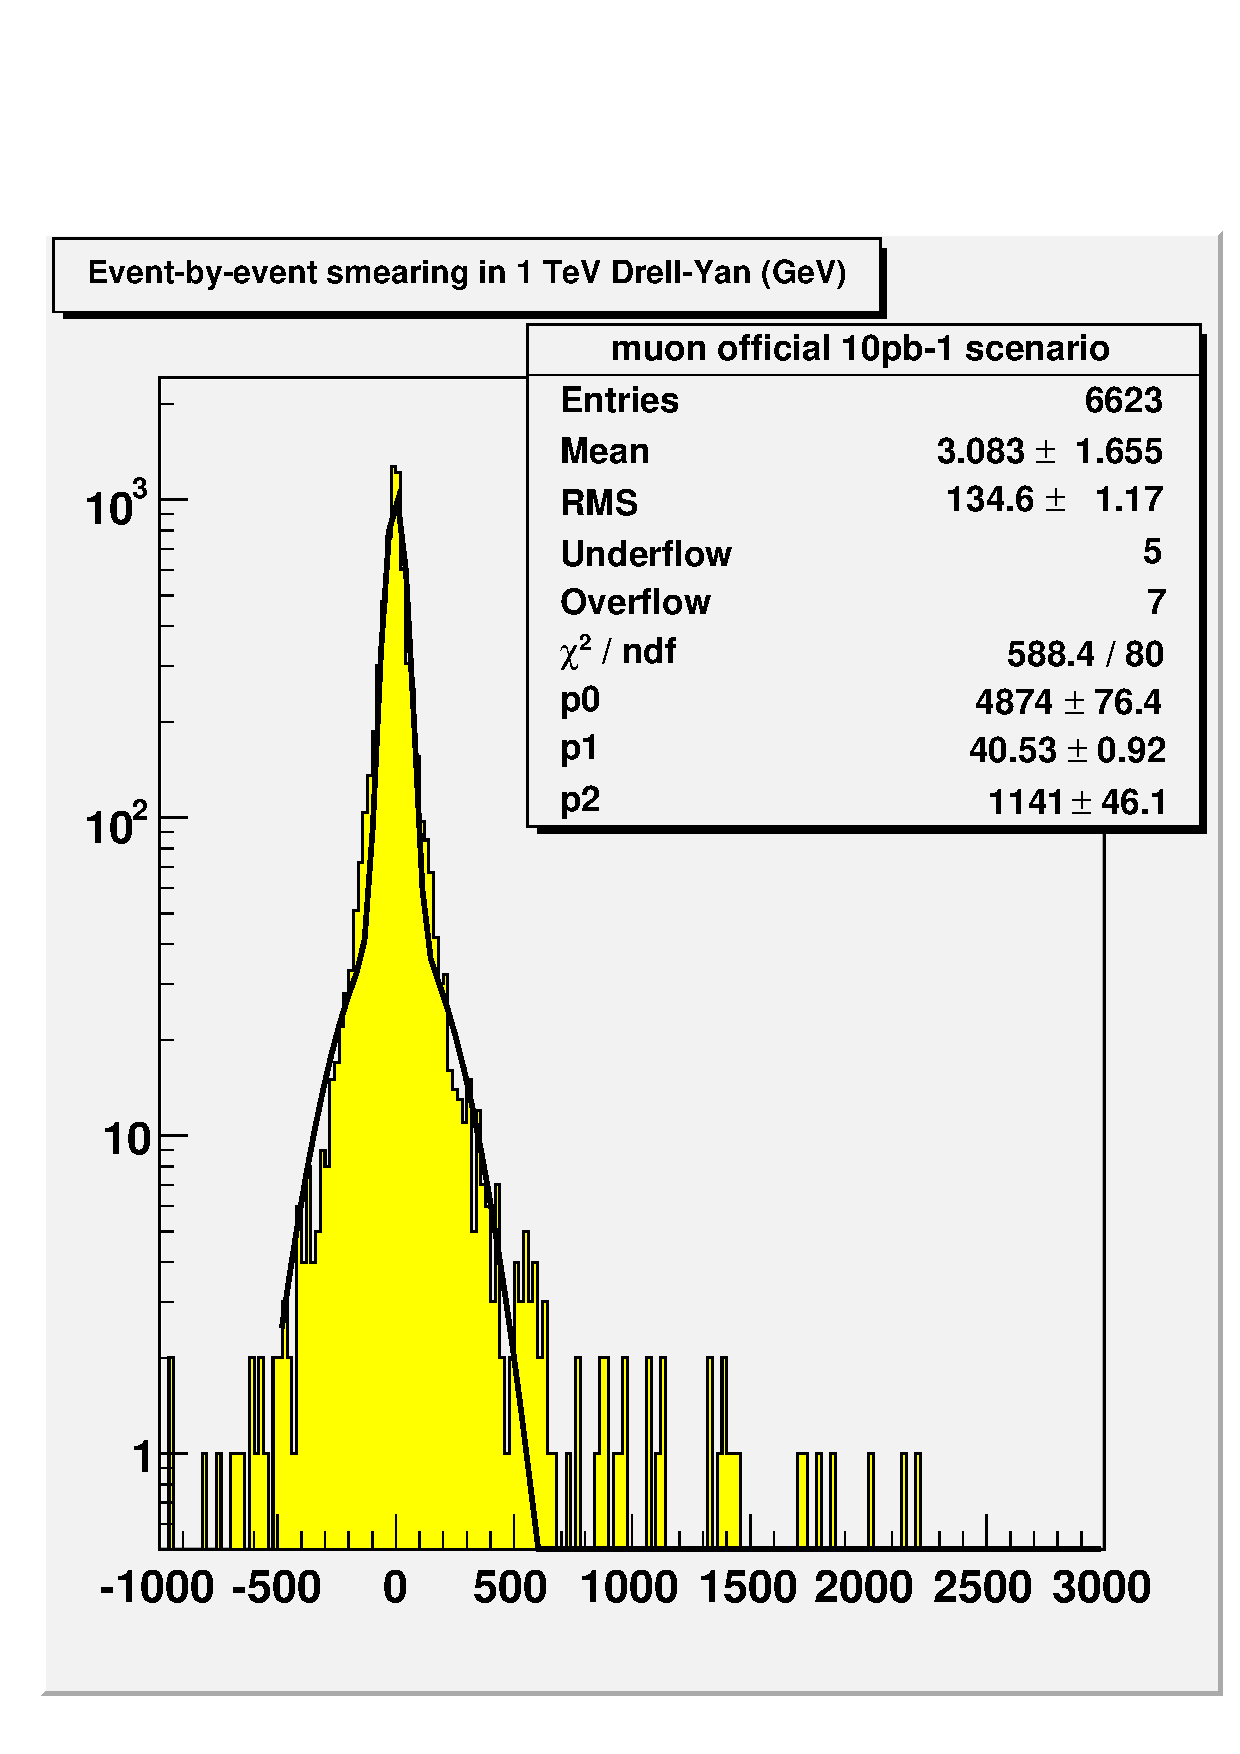
\includegraphics[width=0.33\linewidth]{eventsmear_dy_1000_muonscenario.pdf}
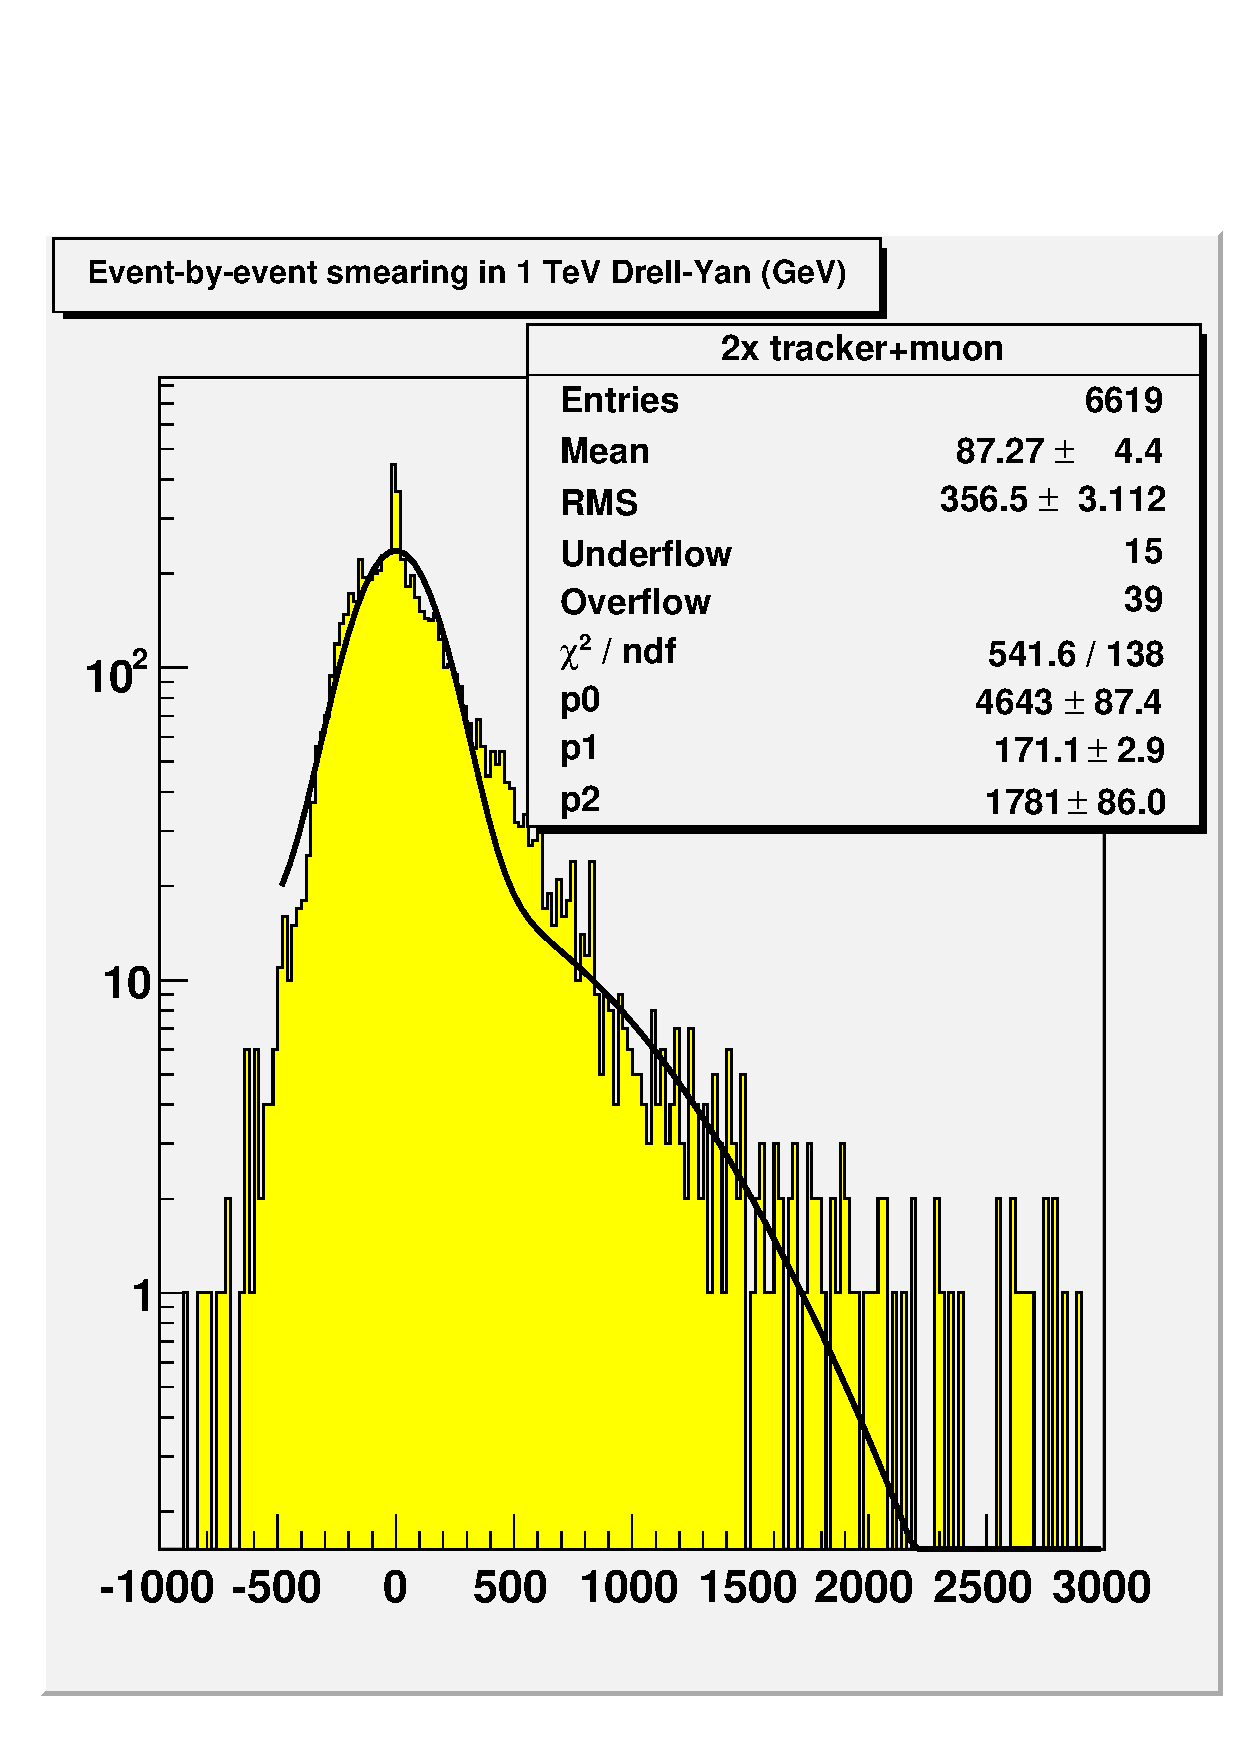
\includegraphics[width=0.33\linewidth]{eventsmear_dy_1000_tracker2.pdf}
\end{center}

\vspace{-0.5 cm}
\begin{itemize}
\item Only in 2$\times$ tracker misalignment scenario does it become significant: $A_i = 0.07$, $\sigma = 500$~GeV, $A_i \, e^{{\sigma_i}^2 k^2 / 2} = 7.3$ 
\item But smearing in this scenario is negligible ($\lesssim 1.5$): when $\Delta E$~$\sim$~500~GeV, $\sigma \to \sigma(E)$, less contribution from low-energy
\item Exponential is cut off by $\sigma(E)$ before it can explode
\end{itemize}
\end{frame}

\begin{notes}
\item For the record, I need to repeat the argument at the bottom of
the last page with more words than would fit.
\item The extreme case (2$\times$ tracker) illustrates a limitation in
the multi-Gaussian model of Drell-Yan convolution.
\begin{itemize}
\item I assumed each Gaussian component had a $\sigma$ which is
constant with respect to energy
\item In reality, the $\sigma$ of each Gaussian $\to$ 0 as $\sqrt{s} \to 0$
\item This effect suppresses the pile-up of low-energy Drell-Yan
events in a given di-muon mass bin to such an extent that the
calculated value of 7 for ``2$\times$ tracker'' is something less than
1.5 (see page 10).
\end{itemize}
\item What we have learned from this exercise is that Drell-Yan falls
off steeply enough ($k$ is small enough) that it will not pile up in
the TeV for even the worst alignments
\item It was a quantitative question that needed to be asked\ldots
\end{notes}

\section*{Resonance broadening}

\begin{frame}
\begin{center}
\Huge \textcolor{blue}{So let's concentrate on resonance broadening}
\end{center}
\end{frame}

\begin{frame}
\frametitle{How much does a misalignment broaden di-muon mass?}
\begin{center}
RMS of event-by-event $\displaystyle \frac{\mbox{misaligned di-muon mass}}{\mbox{ideal di-muon mass}} - 1$
\end{center}

%% 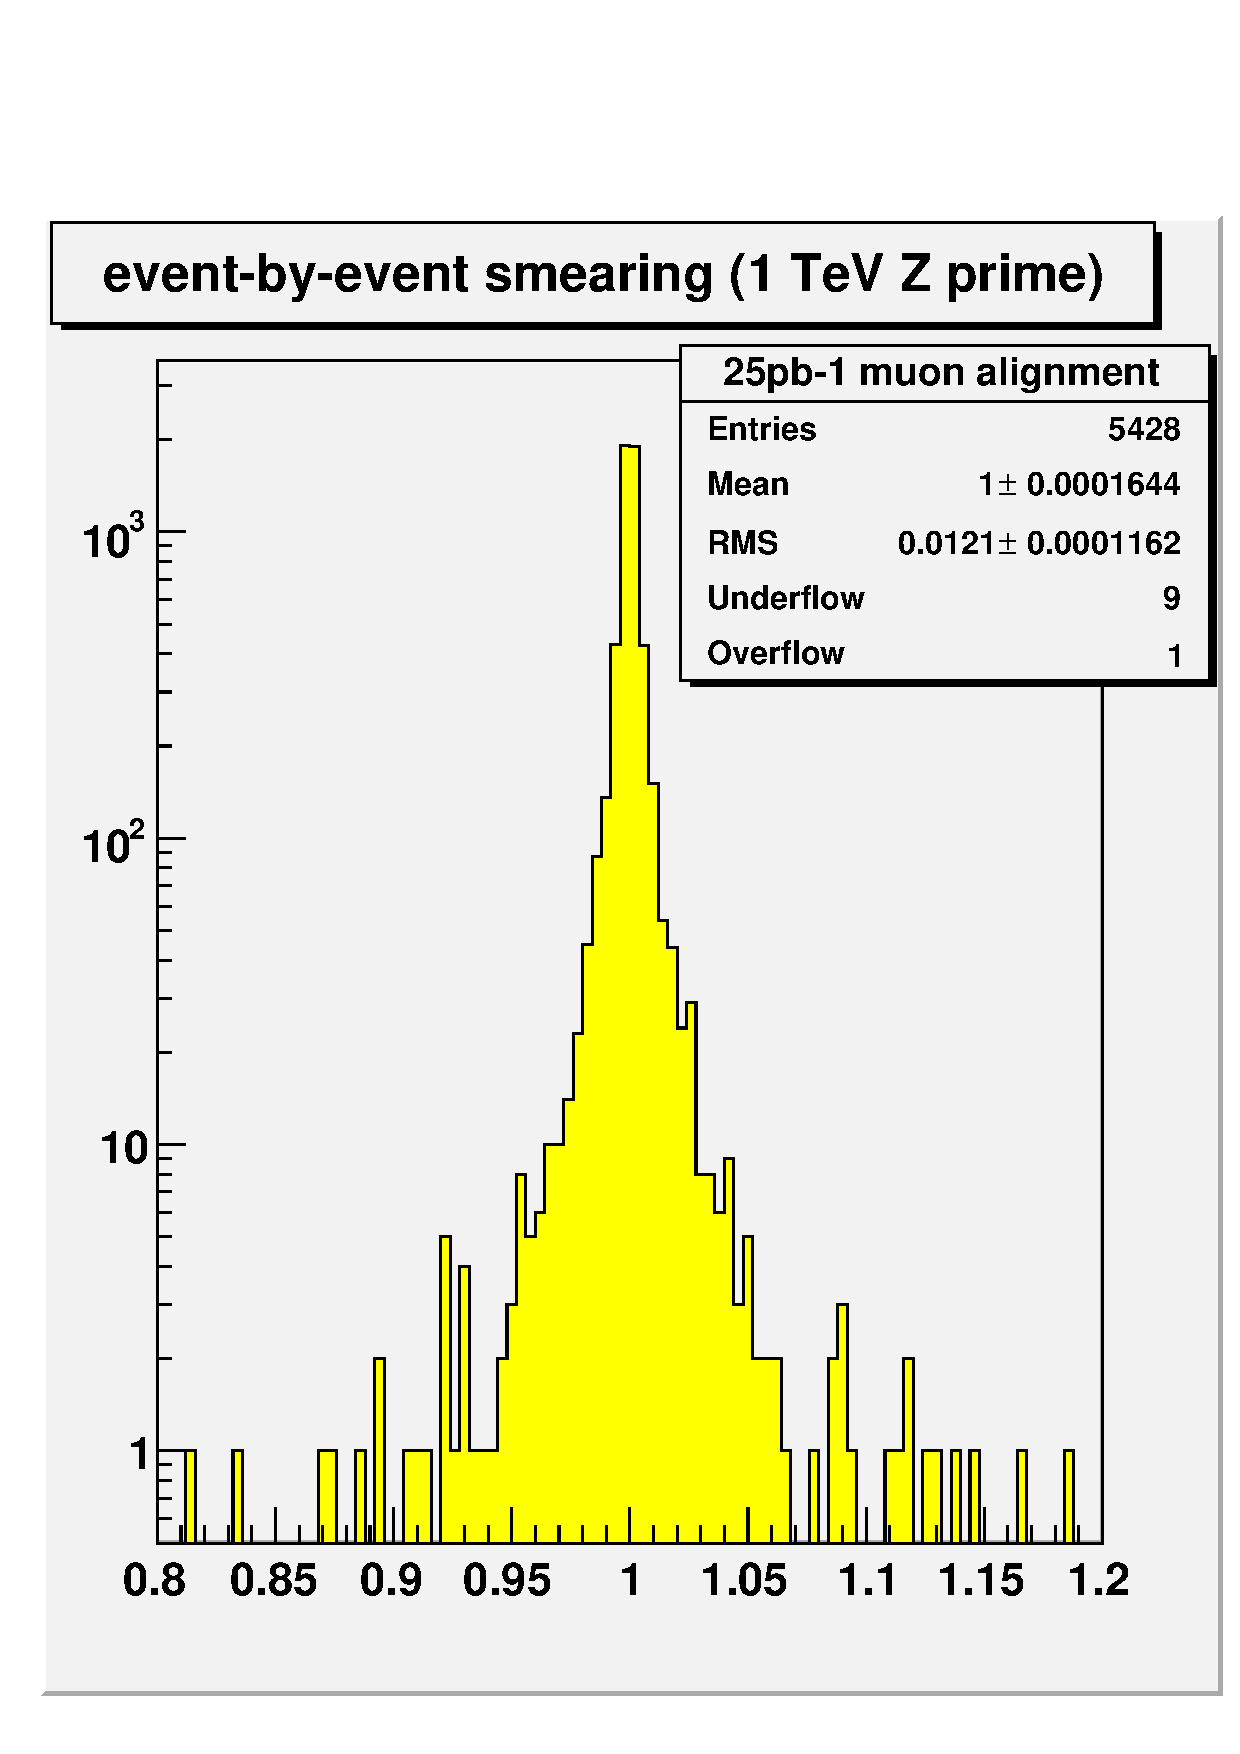
\includegraphics[width=0.25\linewidth]{smearing_events100k.pdf}
%% 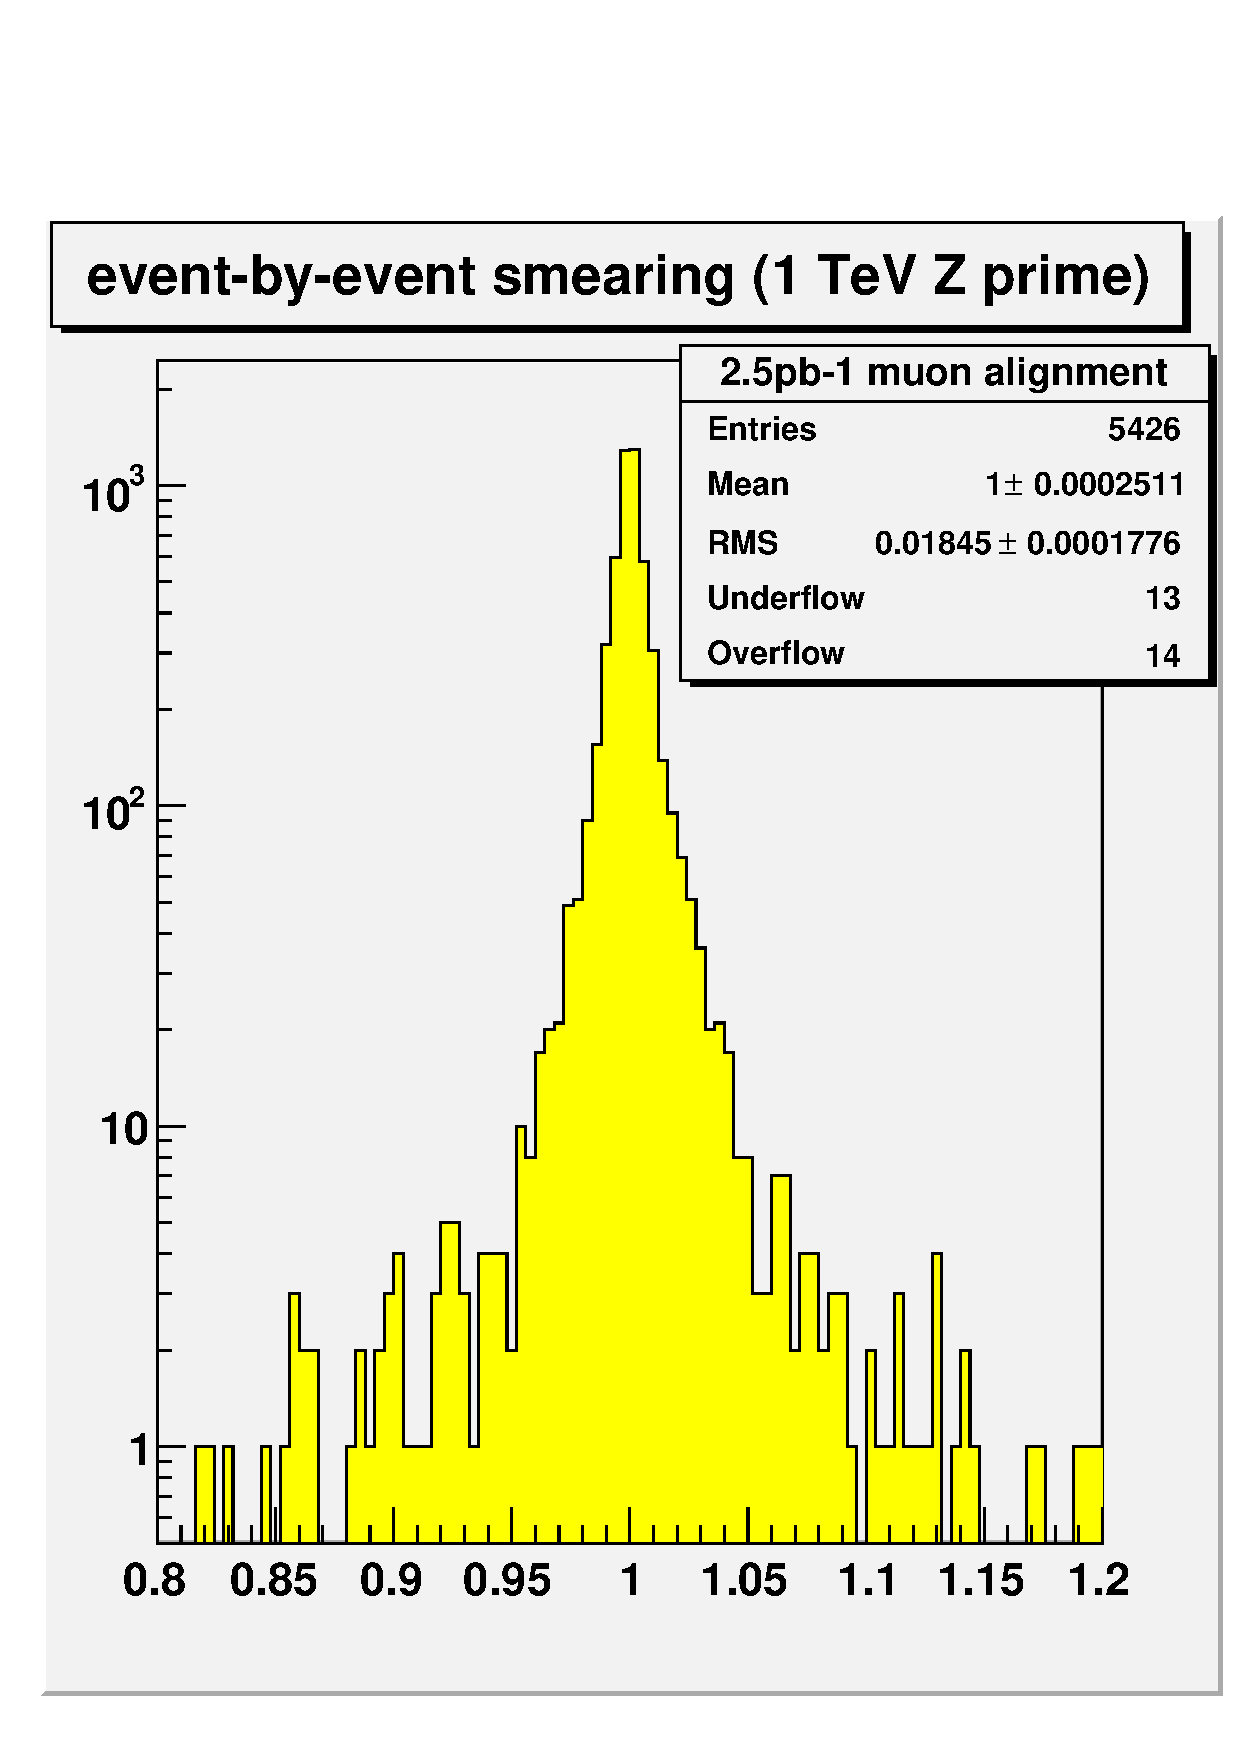
\includegraphics[width=0.25\linewidth]{smearing_events10k.pdf}
\begin{center}
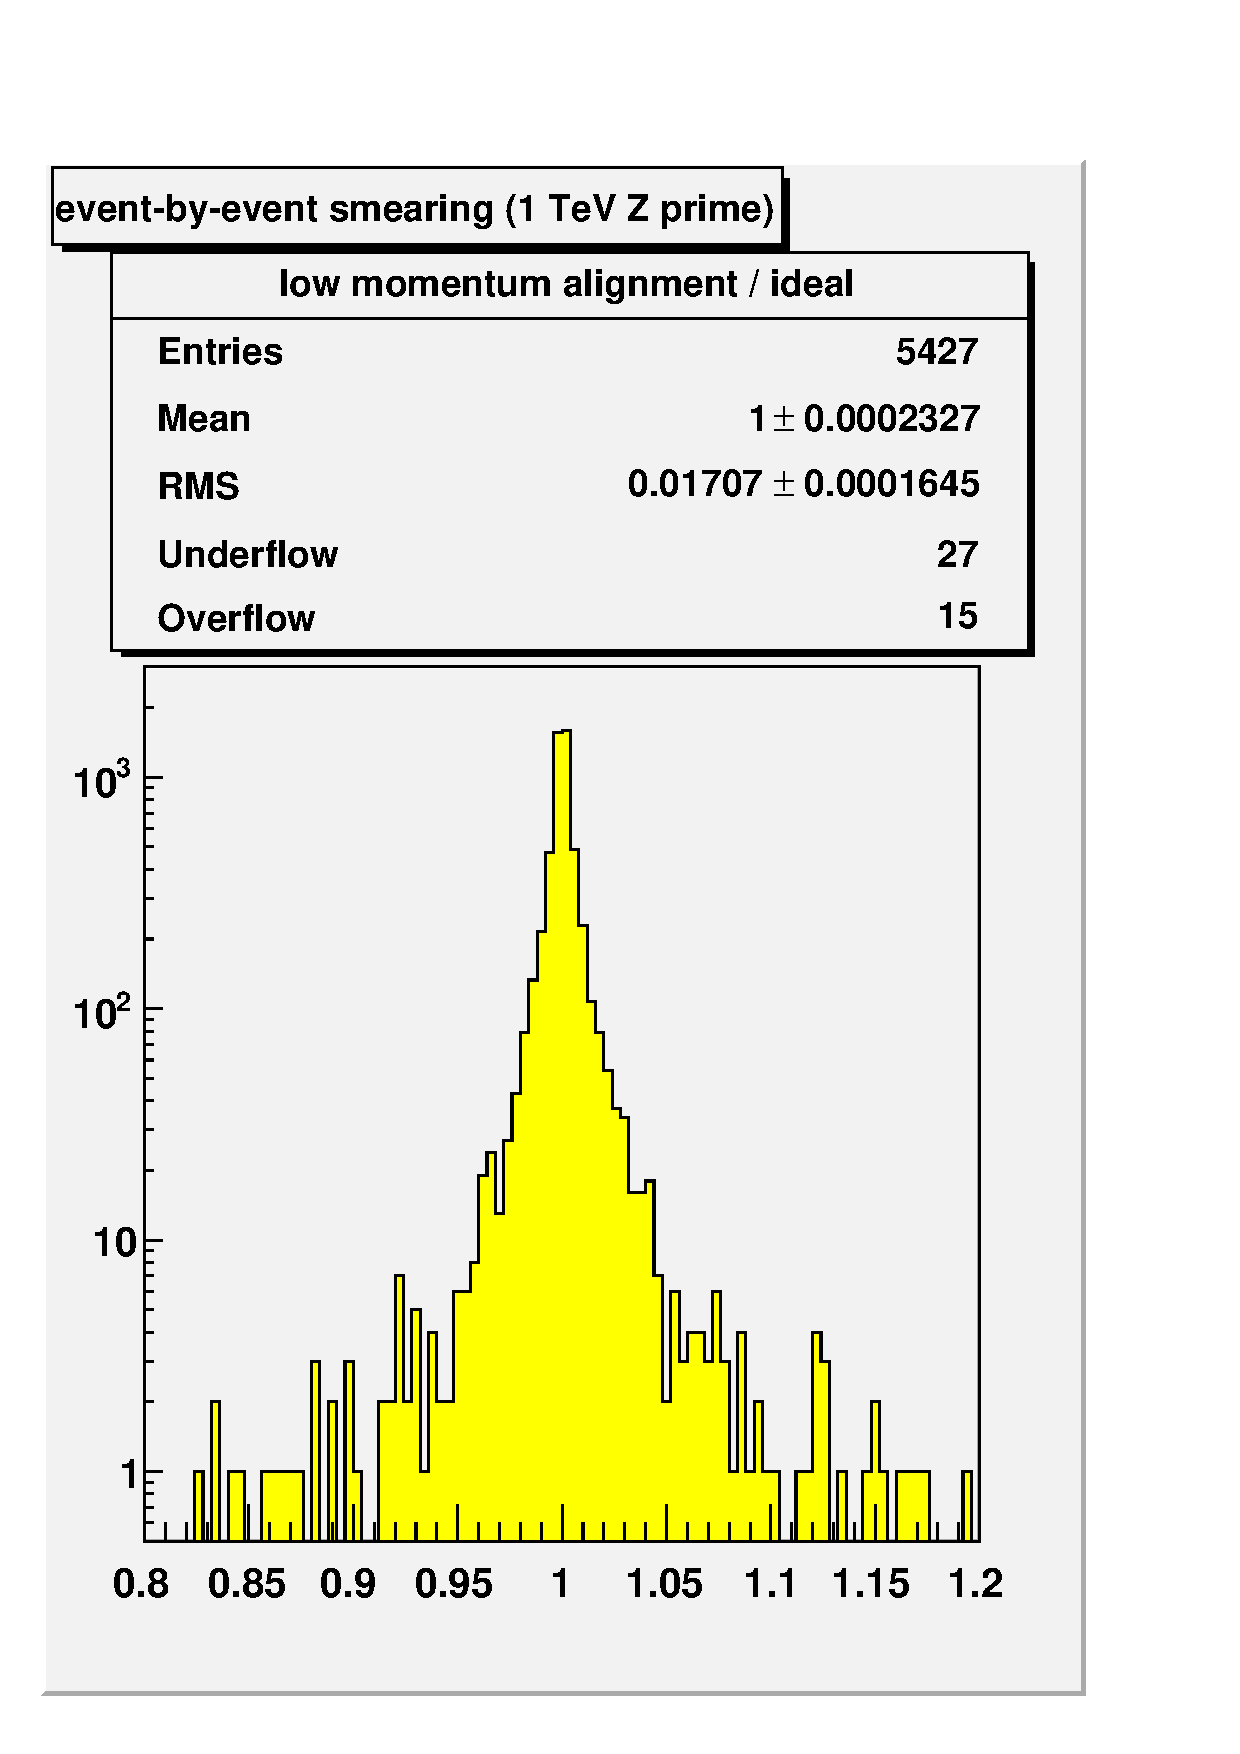
\includegraphics[width=0.35\linewidth]{smearing_momentum_low.pdf}
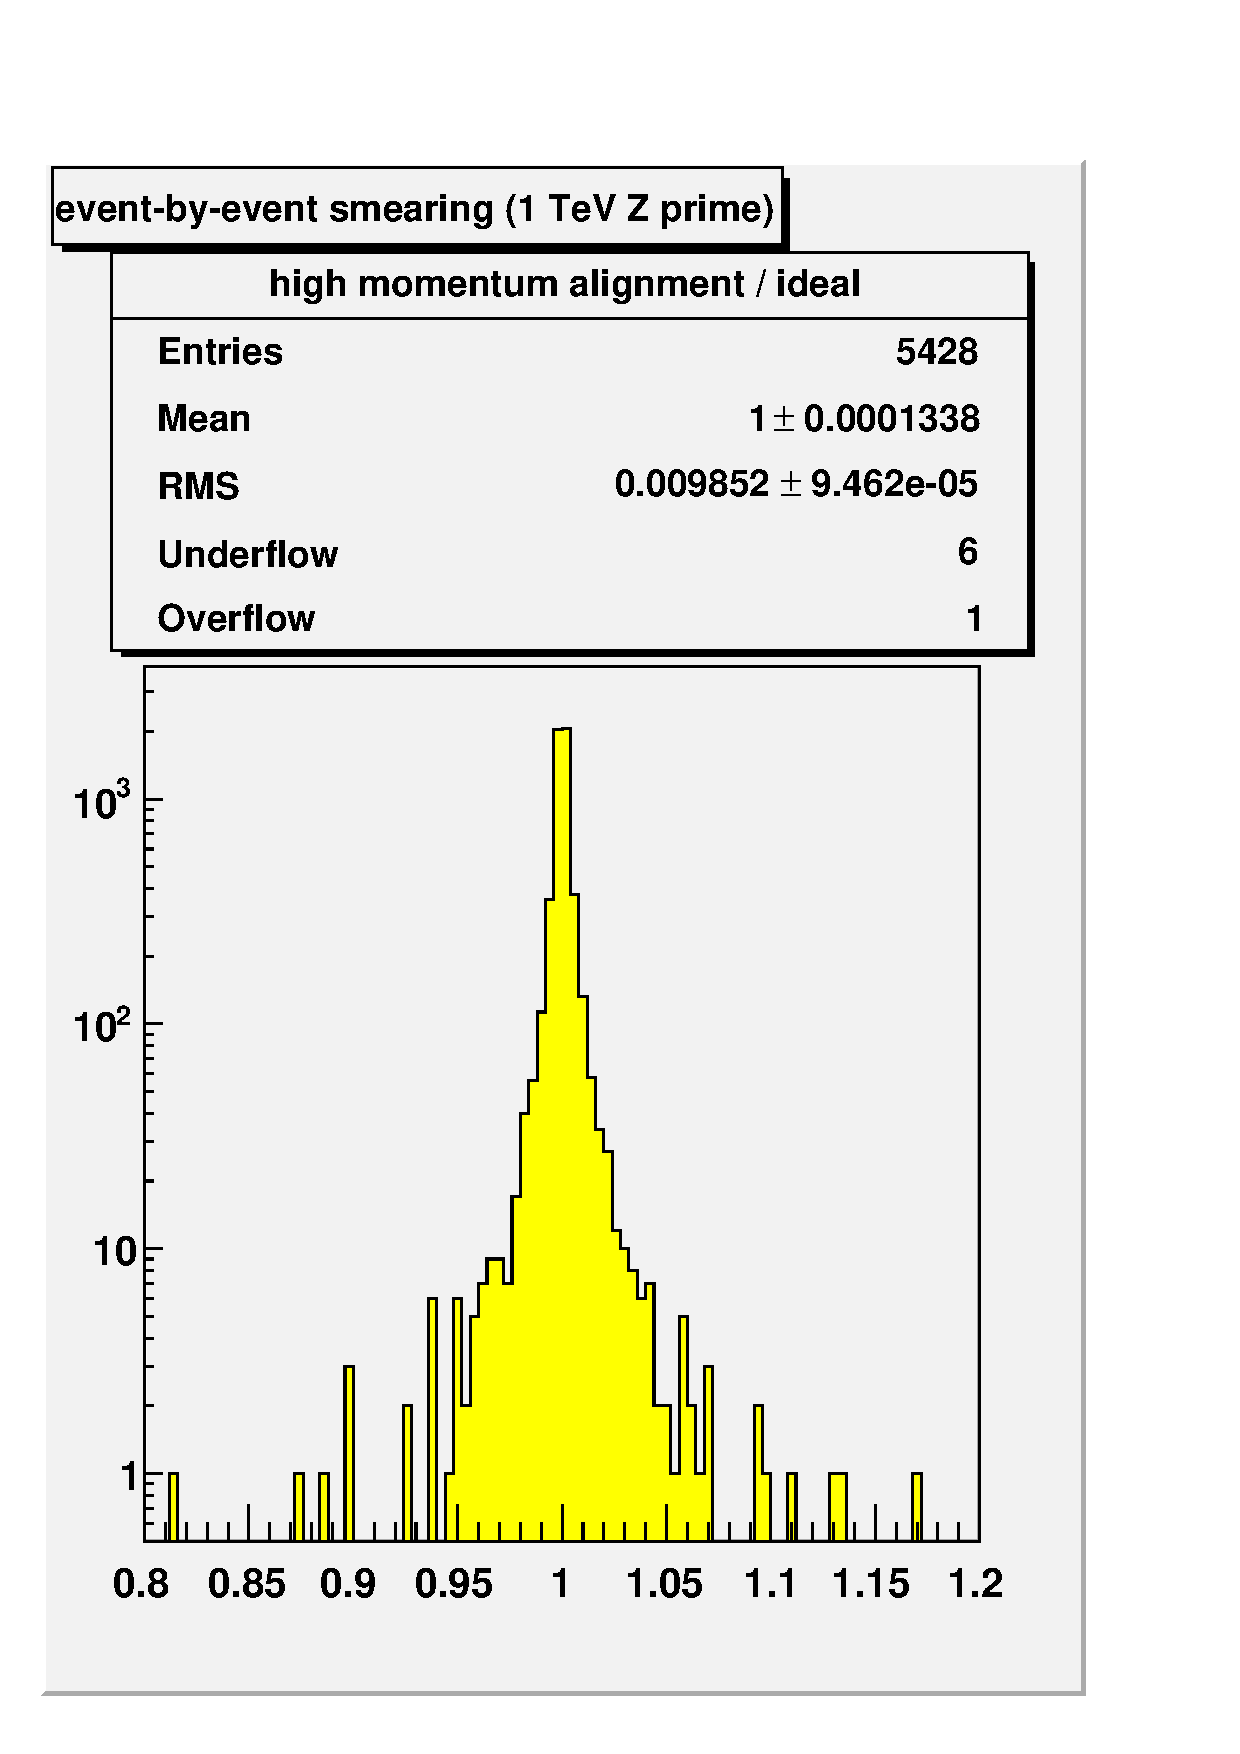
\includegraphics[width=0.35\linewidth]{smearing_momentum_high.pdf}
\end{center}

\underline{\it aligned} with: 20 $<$ $|\vec{p}|$ $<$ 60~GeV \mbox{\hspace{0.65 cm}} $|\vec{p}|$ $>$ 60~GeV \mbox{\hspace{1 cm}}~\mbox{ }
\end{frame}

\begin{notes}
\item This is the same technique as on pages 4 and 5, but applied to di-muon mass instead of track momentum.
\item The {\it same} di-muon mass is observed in an ideal alignment case and a misaligned case.
\item We plot the ratio of these two numbers (minus 1) and take the RMS.
\end{notes}

\begin{frame}
\frametitle{Comparison of alignment scenarios}
\begin{center}
RMS of event-by-event $\displaystyle \frac{\mbox{misaligned di-muon mass}}{\mbox{ideal di-muon mass}} - 1$
\end{center}

\vfill
\renewcommand{\arraystretch}{1.2}
\begin{tabular}{c c c c c}
Source of alignment & $Z'$(1000) & $Z'$(2000) & DY(1000) & DY(2000) \\\hline
1k $\mu$ (0.25~pb$^{-1}$) & 6.0\% & 5.5\% & 4.8\% & 6.6\% \\
10k $\mu$ (2.5~pb$^{-1}$) & 1.8\% & 1.7\% & 1.6\% & 2.1\% \\
100k $\mu$ (25~pb$^{-1}$) & 1.2\% & 1.1\% & 1.0\% & 1.3\% \\
325k $\mu$ (82~pb$^{-1}$) & 1.0\% & 1.0\% & 0.7\% & 1.2\% \\\hline
$|\vec{p}|$ $>$ 60~GeV & 1.0\% & 1.0\% & 0.8\% & 1.2\% \\
20 $<$ $|\vec{p}|$ $<$ 60~GeV & 1.7\% & 1.7\% & 1.5\% & 2.1\%
\end{tabular}

\vfill\vfill With this as a bottom line, we can make statements like
``switching to $|\vec{p}|$ $>$ 60~GeV is as good as getting a factor of
ten more tracks.''
\end{frame}

\begin{frame}
\frametitle{Tails in accuracy from tracker misalignment at high $\eta$}
\begin{columns}
\column{0.7\linewidth}
\mbox{ } \hfill Outer endcap \hfill \hfill Inner endcap \hfill \mbox{ }

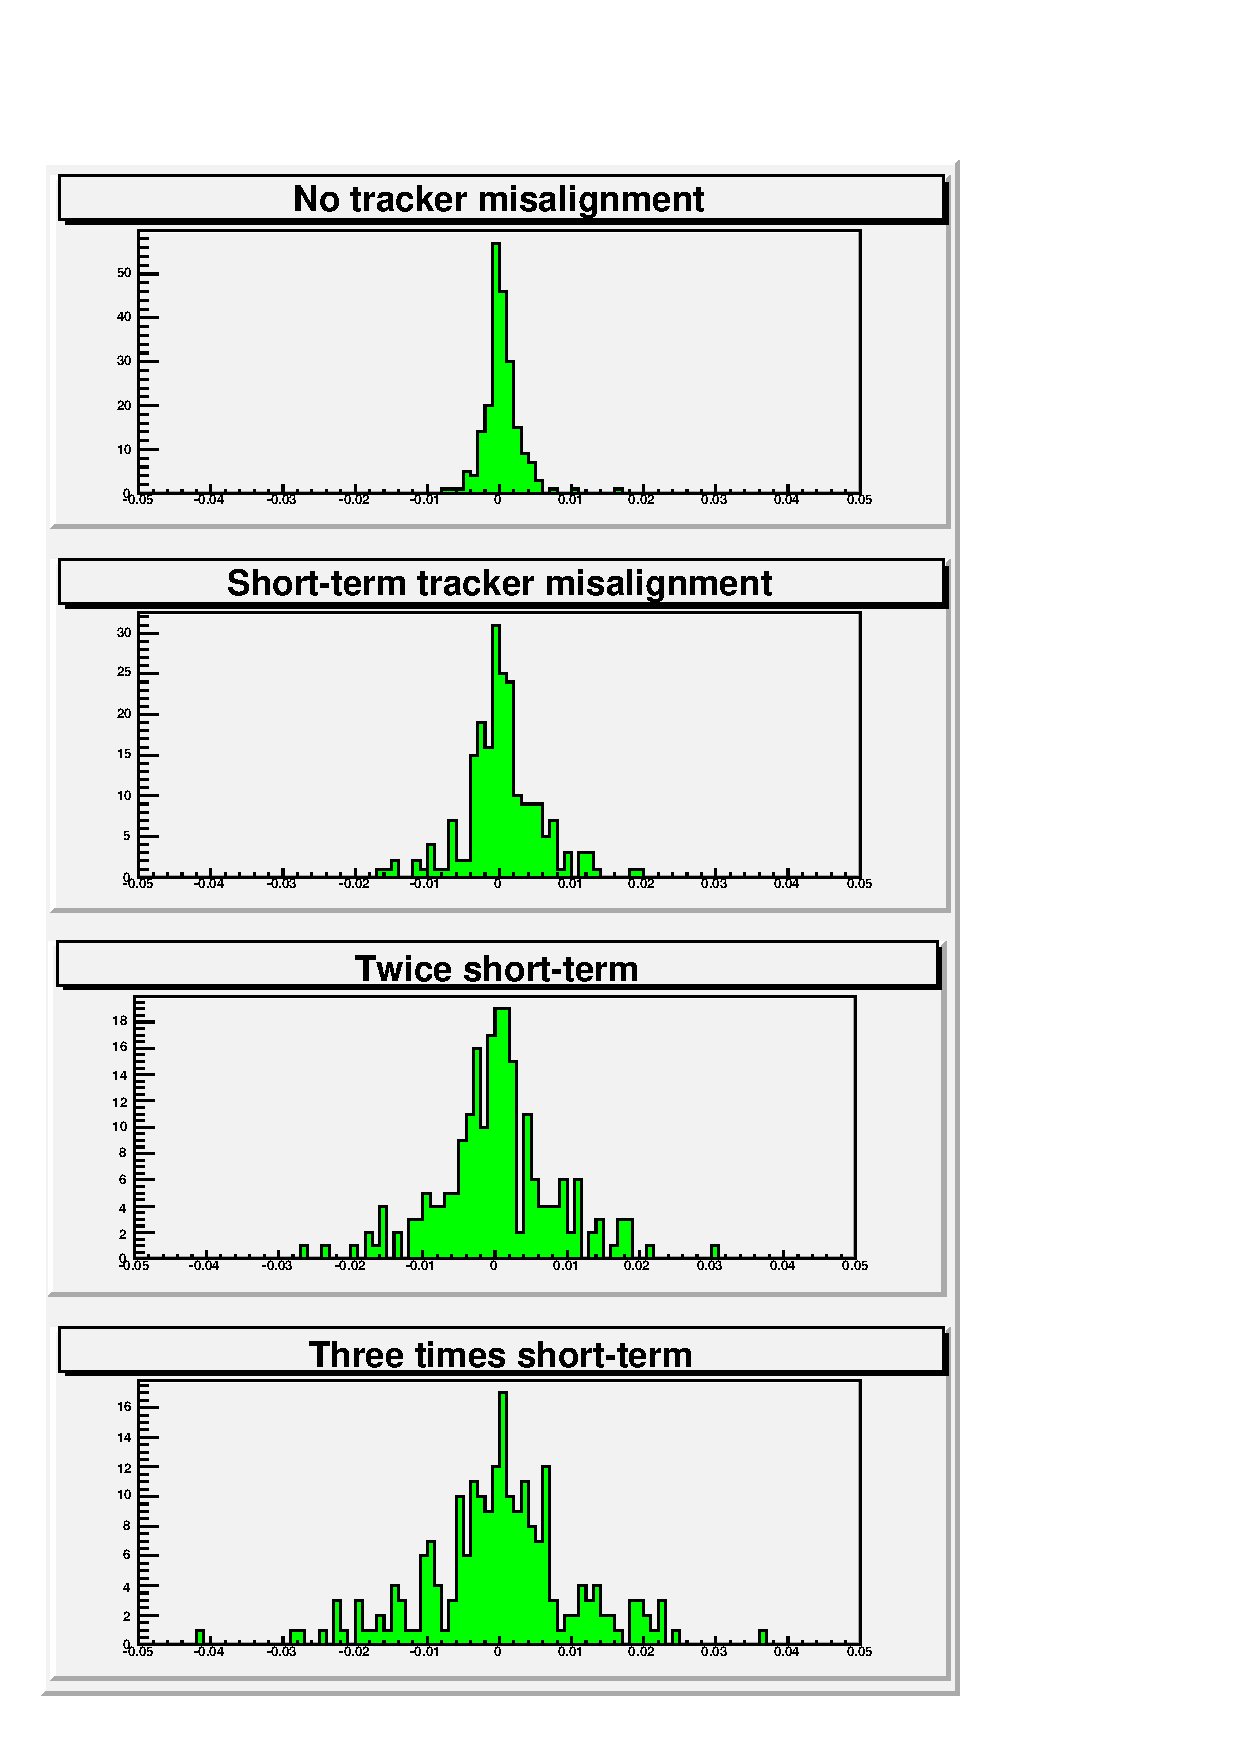
\includegraphics[width=0.5\linewidth]{trackerdep_outer_endcap.pdf}
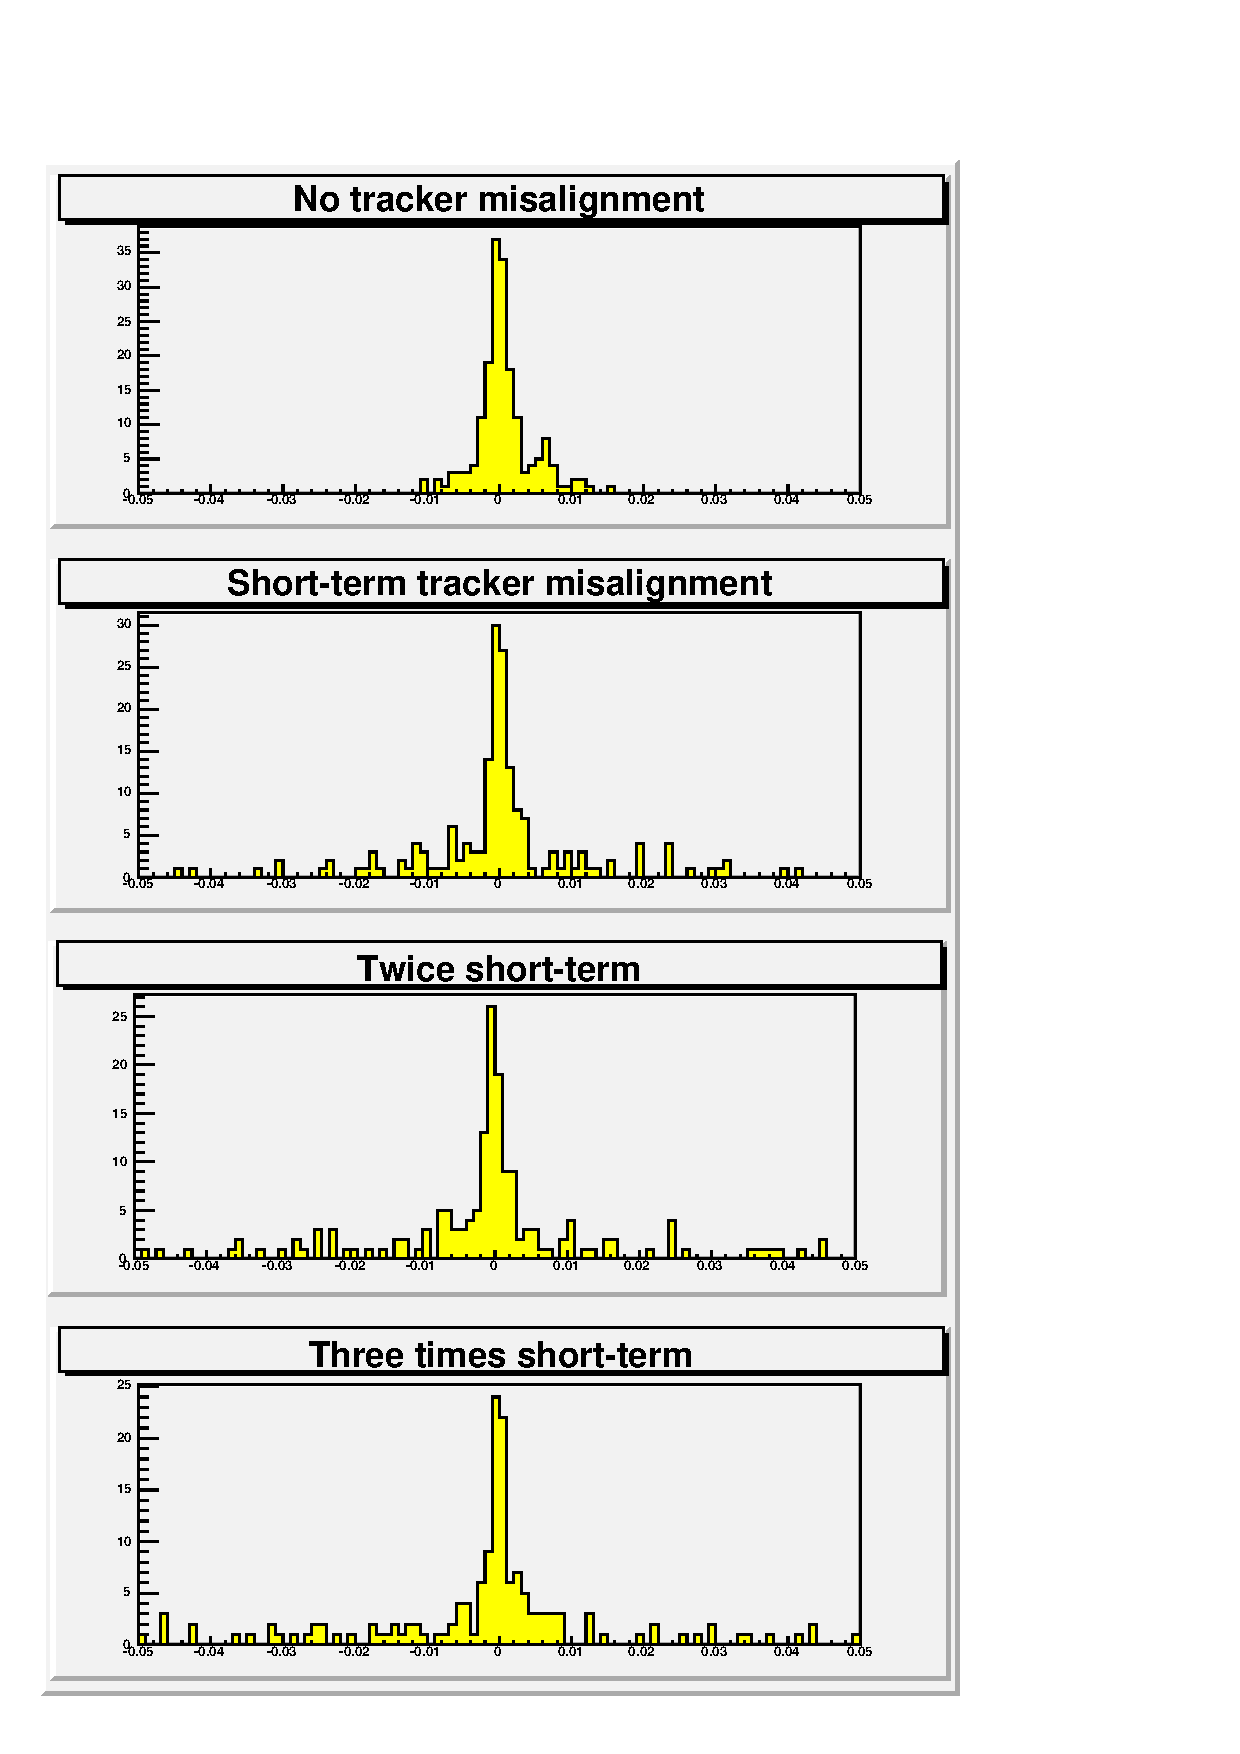
\includegraphics[width=0.5\linewidth]{trackerdep_inner_endcap.pdf}
\column{0.36\linewidth}

\mbox{\hspace{-0.5 cm}} 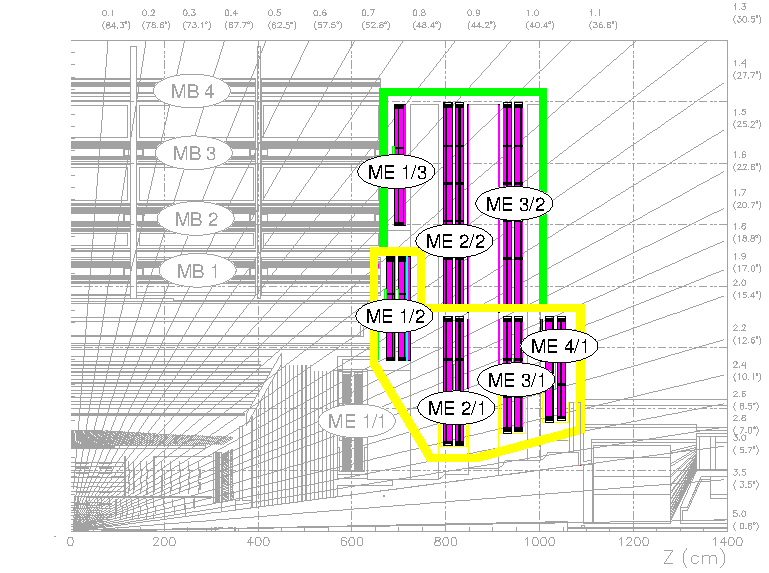
\includegraphics[width=\linewidth]{outer_inner_endcap.pdf}

\vspace{0.2 cm}
Outer endcap (1/3, 2/2, 3/2) only widens

\vspace{0.2 cm}
But inner endcap (1/2, $N$/1) gets more outliers

\end{columns}
\end{frame}

\begin{notes}
\item This is a subtlety of the effect of tracker misalignment on muon
alignment with globalMuons that didn't make it into my EMU talk.
\item Presumably, the tracker misalignment scenario assumes more
misalignment in the TID and TEC regions, the edge of which is at an
$\eta$ of $\sim$1.6.
\end{notes}

\begin{frame}
\frametitle{Effect on di-muons}

\vspace{-1 cm}
\mbox{ }\hfill
\begin{minipage}{0.65\linewidth}
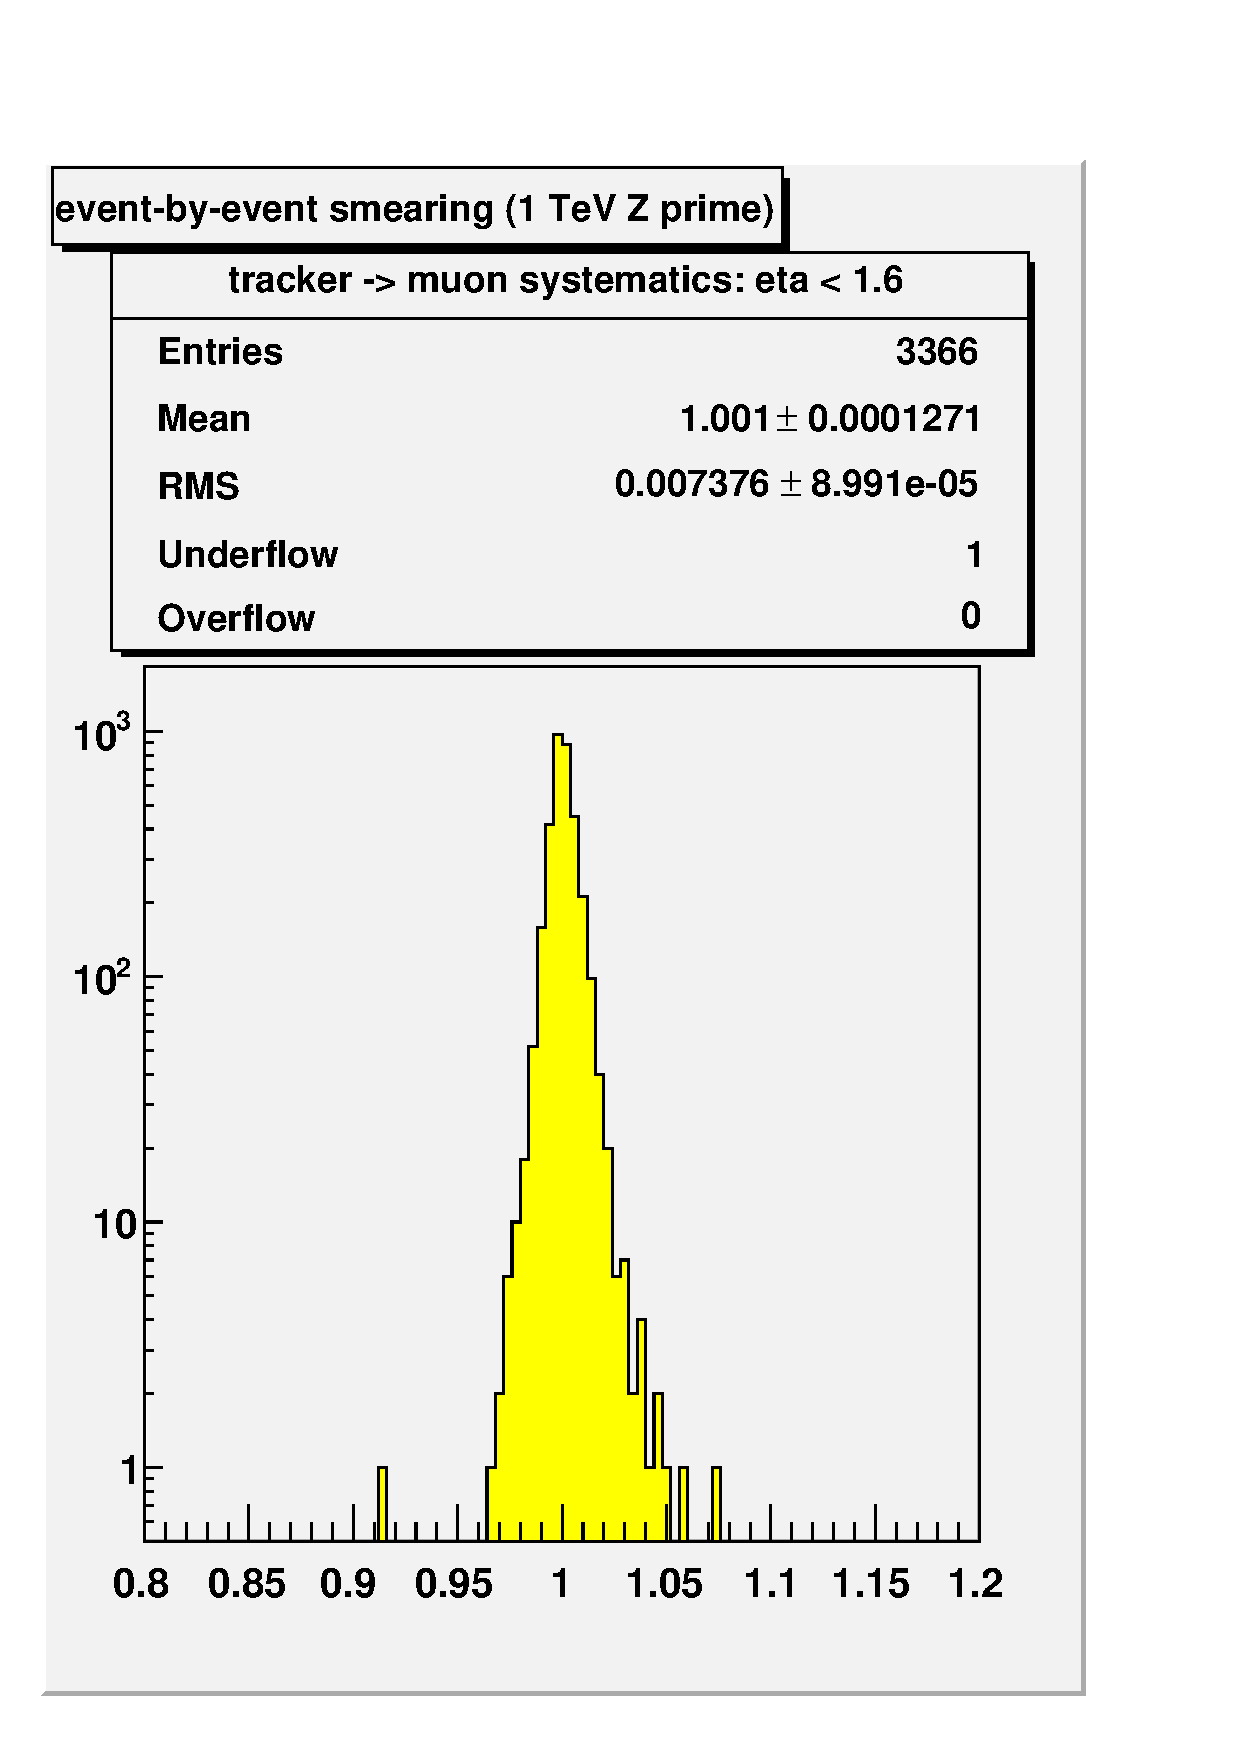
\includegraphics[width=0.5\linewidth]{tracker_systematics_low_eta.pdf}
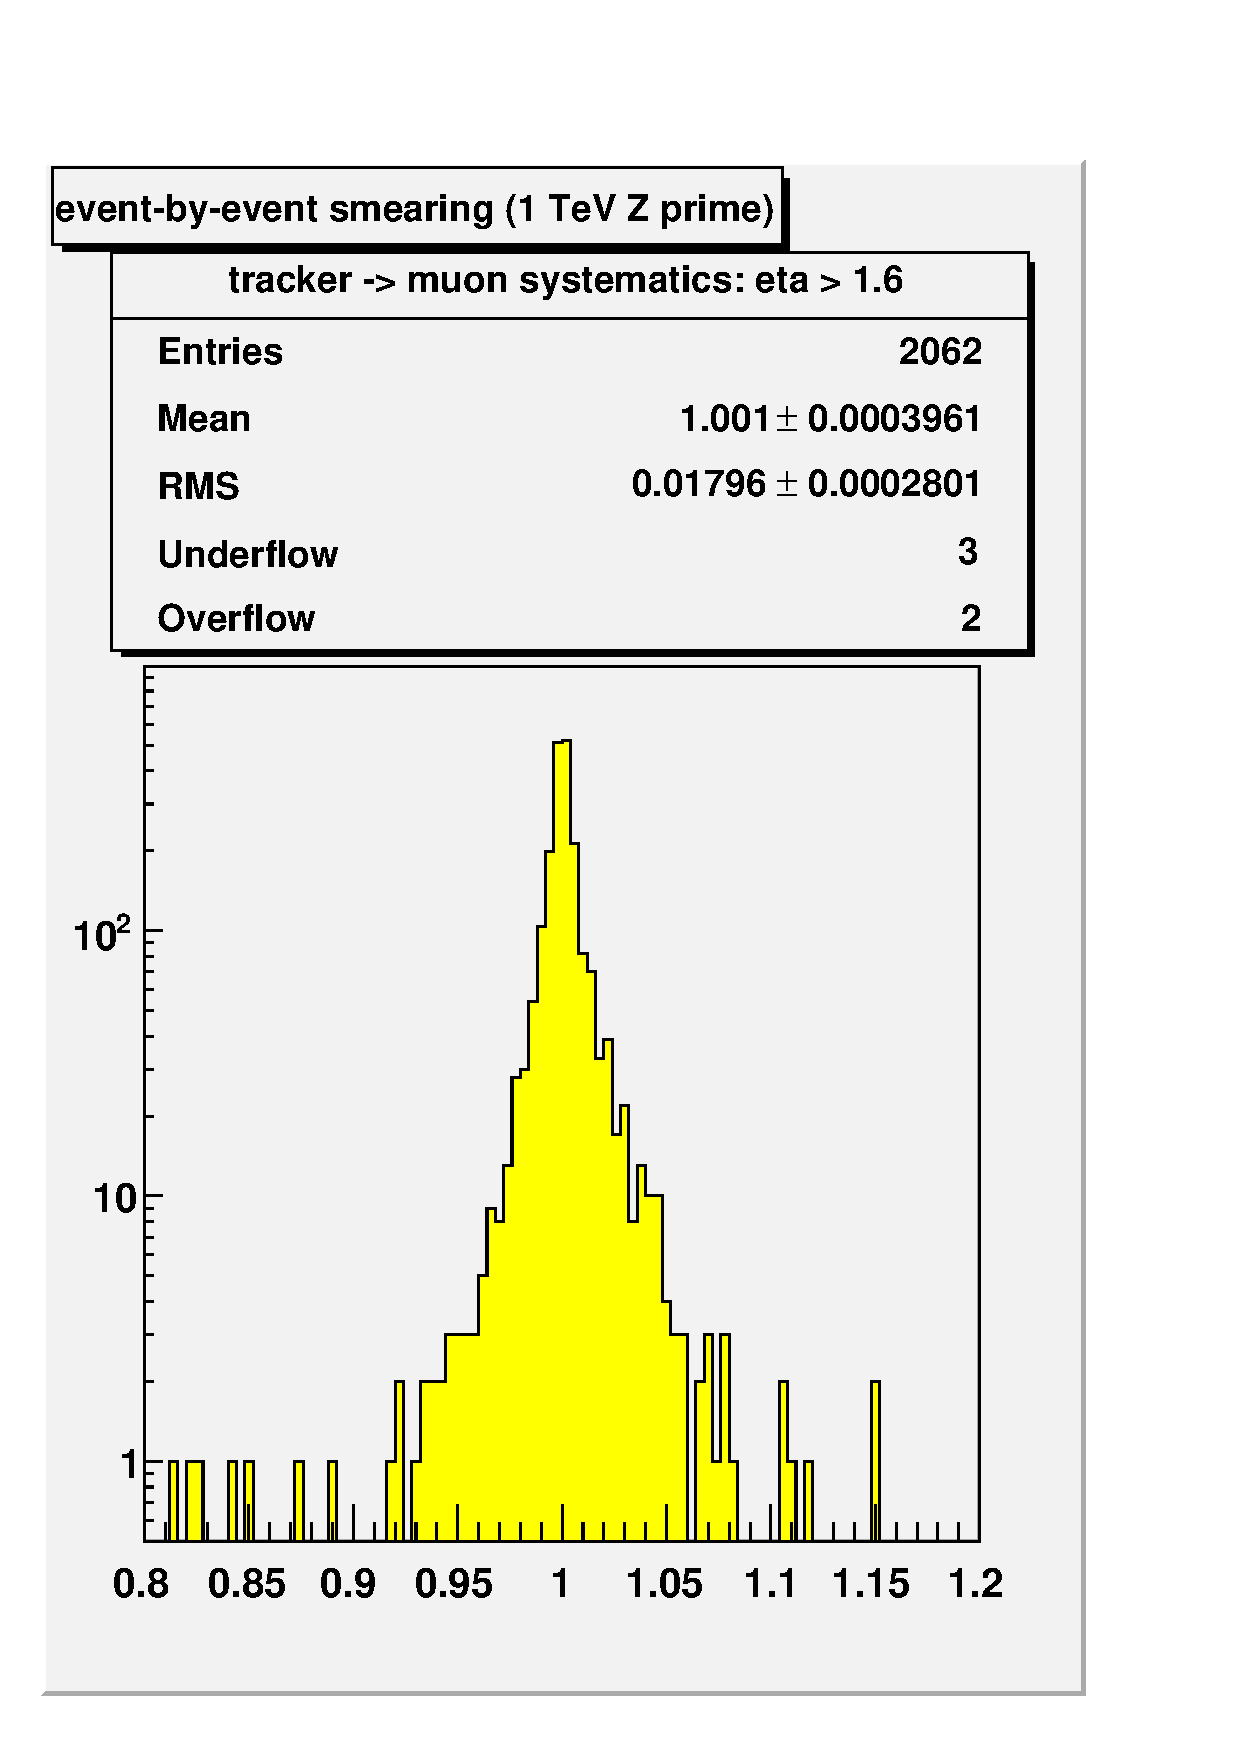
\includegraphics[width=0.5\linewidth]{tracker_systematics_high_eta.pdf}
\end{minipage}

\begin{center}
RMS of $\displaystyle \frac{\mbox{tracker and muon misaligned di-muon mass}}{\mbox{tracker misaligned di-muon mass}} - 1$
\end{center}

\vspace{-0.25 cm}
\renewcommand{\arraystretch}{1.2}
\begin{tabular}{c c c c c}
 & $Z'$(1000) & $Z'$(2000) & DY(1000) & DY(2000) \\\hline
Both $\mu$'s in $|\eta| < 1.6$ & 0.7\% & 0.9\% & 0.5\% & 1.0\% \\
One in $|\eta| > 1.6$ & 1.8\% & 1.5\% & 1.3\% & 2.0\% \\
\end{tabular}
\end{frame}

\section*{\mbox{ }}

\begin{frame}
\frametitle{Conclusions}
\begin{itemize}\setlength{\itemsep}{0.35 cm}
\item Resonance broadening is more significant than Drell-Yan smearing
\item 10~pb$^{-1}$ tracker misalignment {\it scenario} has more
impact on resonance shape (10\%) than 10~pb$^{-1}$ muon alignment {\it scenario} (6\%)
\item Effect of muon misalignment scenario is about 4$\times$ too
pessimistic, including known systematic effects (tracker
extrapolation, momentum dependence down to 20~GeV, miscalibration)
\item Systematic error from tracker extrapolation is measurably larger
in $|\eta| > 1.6$ (2\%) than $|\eta| < 1.6$ (1\%).
\end{itemize}
\label{numpages}
\end{frame}

\end{document}
